\documentclass[a4paper,12pt]{scrreprt}
    %% Used for changing geometry of the page
    %% Cover page text cannot overlay cover sketching/style
    %% https://ctan.org/pkg/geometry?lang=en
\usepackage{geometry}
    %% Changes language of some packages protocols
    %% e.g., when captioning images: Figure 1. -> Figura 1.
    %% https://ctan.org/pkg/babel?lang=en
\usepackage[portuguese]{babel}
    %% Used for special fonts
    %% Cannot be compiled with pdflatex
    %% https://ctan.org/pkg/fontspec?lang=en
\usepackage{fontspec}
    %% Arial FONT
    \setmainfont{Arial}
    %% More colors and color options
    %% https://ctan.org/pkg/xcolor?lang=en
    %% https://ctan.org/pkg/colortbl?lang=en
\usepackage{xcolor,colortbl}
    %% More tabular options, like dashed/dotted lines
    %% https://ctan.org/pkg/arydshln?lang=en
\usepackage{arydshln}
    %% List of acronyms
    %% https://ctan.org/pkg/nomencl?lang=en
\usepackage[intoc]{nomencl}
    %% Must be called to init nomencl environment
    \makenomenclature
    %% More images options/settings
    %% https://ctan.org/pkg/graphicx?lang=en
\usepackage{graphics}
    %% Defining subdirectories to image path enviornment
    %% \graphicspath{{sub1}{sub2}...{subN}}
    \graphicspath{{images}}

    %% used to handle cross-referencing commands in LaTeX to produce hypertext links in the document
    %% https://ctan.org/pkg/hyperref?lang=en
\usepackage{hyperref}
    %% math environments
    %% https://ctan.org/pkg/amsmath?lang=en        
    %% settings
    \hypersetup{
        colorlinks,
        citecolor=black,
        filecolor=black,
        linkcolor=black,
        urlcolor=black
    }

\usepackage{amsmath}
    %% Defining backgrouns, used to make the cover
    %% https://ctan.org/pkg/background?lang=en
\usepackage[some]{background}
    %% Used to make drawings or complex graphics
    %% http://pgf.sourceforge.net/pgf_CVS.pdf
\usepackage{tikz}
    %% Tikz library to point operations ((x1,y1) + (x2,y2))
    \usetikzlibrary{calc}

%% code snippets
\usepackage{listings}
\usepackage{color}

\definecolor{dkgreen}{rgb}{0,0.6,0}
\definecolor{gray}{rgb}{0.5,0.5,0.5}
\definecolor{mauve}{rgb}{0.58,0,0.82}

\lstset{
    frame=tb,
    language=SQL,
    aboveskip=3mm,
    belowskip=3mm,
    showstringspaces=false,
    columns=flexible,
    basicstyle={\small\ttfamily},
    numbers=left,
    numberstyle=\small\color{gray},
    keywordstyle=\color{blue},
    commentstyle=\color{dkgreen},
    stringstyle=\color{mauve},
    breaklines=true,
    breakatwhitespace=true,
    tabsize=3,
    moredelim=**[is][\color{blue}]{@}{@}
}

%% further RelaX definitions
%% \usepackage{stix}

%% Defining sfdefault font and default font for document
\renewcommand{\familydefault}{\sfdefault}

%% For tables
\usepackage{pbox}
\usepackage{longtable}
\usepackage{xcolor} % for coloring rows
\usepackage{multirow}
\usepackage{hhline}
\usepackage{array}

% Custom ColumnSpec for tables
% \newcolumntype{ColumnSpec}{|p{0.3cm}|p{4cm}|p{3cm}|p{4.5cm}|p{3cm}|}
\newcommand{\MyColumnSpec}{|p{0.3cm}|p{4cm}|p{3cm}|p{4.5cm}|p{3cm}|}

%% Rquisitos table header custom command
\newcommand{\Header}[1]{%
    \hline
    \rowcolor{#1} \cellcolor{#1} Nr & \multicolumn{4}{c|}{\cellcolor{#1}Descrição} \\
    \hhline{~----}
    \cellcolor{#1}
    & \cellcolor{#1}Data e Hora & \cellcolor{#1}Área & \cellcolor{#1}Fonte & \cellcolor{#1}Analista \\
    \hline
}

%% Custom commands for filling cells
\newcommand{\Nao}{%
    \cellcolor{red!40}Não
}
\newcommand{\Sim}{%
    \cellcolor{green!40}Sim
}
\newcommand{\Maybe}{%
    \cellcolor{yellow!40}Talvez
}
%==========================================================================
% DOCUMENT
%==========================================================================

\begin{document}

\pagenumbering{gobble}

%% Costume made cover
%% From there you can use \makecover command to build the cover
%% Blue cover color
\definecolor{titlepagecolor}{RGB}{54,95,145}

%==========================================================================
% COLORED BAR ON THE LEFT SIDE
%==========================================================================

\backgroundsetup{
    scale=1, 
    angle=0, 
    opacity=1,
    contents={
        \begin{tikzpicture}[remember picture,overlay]
            \path [fill=titlepagecolor] 
                (current page.north west) -- ($(current page.north west) + (5,0)$)
                -- ($(current page.south west) + (5,0)$)-- (current page.south west); 
            \node[color=white] at ($(current page.south west) + (3,4)$) {\bfseries {\fontsize{120}{60} \textsf{LI}}};
            \node[color=titlepagecolor] at ($(current page.south west) + (5.8,4)$) {\bfseries {\fontsize{120}{60} \textsf{4}}};
        \end{tikzpicture}
    }
}

%==========================================================================
% TITLE PAGE INFO
%==========================================================================

%% Changes values in this field to show information in the cover and back cover about your team/project


%% TITLE
\title{CDC – Consultoria de Detetives Christie}

%% AUTHORS
\author{
    Afonso Dionísio Santos (A10426) \\
  \quad
    Ana Filipa Cruz Pinto (A96862) \\
  \quad
    Carlos Humberto da Silva Ferreira (A89509) \\
  \quad
    Flávia Alexandra Silva Araújo (A96587) \\
  \quad
    Miguel Torres Carvalho (A95485)
}

%% Date

\date{\today}

%% Course
\newcommand{\Course}{Licenciatura em Engenharia Informática}

%% Department
\newcommand{\Department}{Escola de Engenharia}

%% UniName
\newcommand{\UniName}{Universidade do Minho}

%% UniPic
\newcommand{\UniPic}{
\includegraphics[scale=0.09]{images/uminho.png}}

%% University 
\newcommand{\University}{
    \begin{flushleft}
        \UniPic
    \end{flushleft}
    \textcolor{gray}{\small\textbf{\textsf{\UniName}}}\par
    \textcolor{gray!80!white}{\small{\textsf{\Department}}}\par
    \textcolor{gray!70!white}{\small{\textsf{\Course}}}
}

%% UC
\newcommand{\UC}{
    \begin{flushleft}
        \par\textcolor{titlepagecolor}{  \LARGE\textbf{\textsf{Unidade Curricular de \\ Laboratórios de Informática IV}}}
    \end{flushleft}
}

%% School Year
\newcommand{\SchoolYear}{
    \small{\textsf{Ano Letivo de 2023/2024}}}


%% Define new command to show title, author and date
\makeatletter
\let\Title\@title
\let\Author\@author
\let\Date\@date
\makeatother

%==========================================================================
% CLASSIFICATION SECTION 
%==========================================================================

%% School Year
\newcommand{\ReceptionDate}{}
%% Responsible
\newcommand{\Responsible}{}
%% Evaluation
\newcommand{\Evaluation}{}
%% Observations
\newcommand{\Observations}{}





%% MAKETEMPLATE
\newcommand{\makecover}{

%==========================================================================
% BEGIN COVER PAGE 
%==========================================================================

%% Removes page number on footer
\thispagestyle{empty}

%% No indentation 
\setlength{\parindent}{0em}

%% Put Background defined on \backgroundsetup, in this page
\BgThispage

%% Changing geometry to prevent overlay with text
%% At the end of back cover, geometry is default with \restoregeometry
\newgeometry{top=5cm,left=6cm,right=3cm,bottom=2cm}

%% builds university info defined previously
\University
\vspace{1cm}
%% builds curricular unity info defined previously
\UC
%% builds school year info defined previously
\SchoolYear

\vspace*{5cm}
%% bigger space (i think its the default one) between paragraphs 
\setlength{\parskip}{1em}

%% builds title info defined previously
\par\textbf{\textsf{\huge\Title}}
\vspace{1cm}
%% builds author(s) info defined previously
\par\Author

\vspace{0.5cm}

%% builds date info defined previously
\par\Date
\restoregeometry
\pagebreak

%==========================================================================
% END COVER PAGE 
%==========================================================================

%==========================================================================
% BEGIN BACK COVER PAGE 
%==========================================================================

%% Removes page number on footer
\thispagestyle{empty}

% Changing look of lines in tabular environment 
% Dashed -> dotted 
%% length of dashes
\setlength\dashlinedash{0.3pt}
%% space between dashes
\setlength\dashlinegap{1.5pt}
%% width of dashes
\setlength\arrayrulewidth{1.1pt}


%% This values can be changed in the preamble
\begin{flushright}
\begin{tabular}{ :p{4cm}:p{4cm}: } 
\hdashline
Data de Receção & \ReceptionDate \\ [2ex]
\hdashline
Responsável & \Responsible \\ [2ex]
\hdashline
Avalição & \Evaluation \\ [2ex]
\hdashline
Observações & \Observations \\ [7ex]
\hdashline
\end{tabular}
\end{flushright}


\vspace{9cm}
\begin{flushleft}

%% builds title info defined previously
\par\textbf{\textsf{\huge\Title}}
\vspace{1cm}
%% builds author info defined previously
\par\hspace{0.25cm}\Author

\vspace{0.5cm}

%% builds date info defined previously
\par\Date
\end{flushleft}

\pagebreak
%==========================================================================
% END BACK COVER PAGE 
%==========================================================================
}


% builds the cover
\makecover

%% smaller footer and header size
\newgeometry{top=3cm,left=3cm,right=3cm,bottom=4cm}
\savegeometry{default}

%==========================================================================
% BEGIN OPCIONAL DEDICATÓRIA
%==========================================================================

% \clearpage
% \begin{center}
%     \thispagestyle{empty}
%     \vspace*{\fill}
%
%     $<<$/opcional Dedicatória$>>$
%
%     \vspace*{\fill}
% \end{center}
% \clearpage

%==========================================================================
% END OPCIONAL DEDICATÓRIA
%==========================================================================

%==========================================================================
% BEGIN ABSTRACT PAGE
%==========================================================================

%% Abstract name: \Large font size, flushed left and paragraph skip before abstract content
\renewenvironment{abstract}
 {\par\noindent\textbf{\Large\abstractname}\par\bigskip}
 {}

\begin{flushleft}
\begin{abstract}
    No âmbito da UC Base de Dados, lecionada pelo regente, Professor Orlando Belo, visamos a
    realização de um projeto que consiste na modelação, desenvolvimento e implementação de um
    Sistema de Base de Dados Relacional.
    
    Tendo em consideração o tema deste ano - uma agência de detetives -, decidimos explorar
    uma agência liderada por Agatha Christie, de nome CDC - Consultoria de Detetives Christie.
    Relativamente à modelação e desenvolvimento do nosso projeto, iremos dividi-lo em partes: começaremos de forma abstrata e de alto nível, transformando os factos em requisitos e fazendo uma progressão sucessiva para um baixo nível à medida que convertemos estes num modelo conceptual, e, por conseguinte, o conceptual num modelo lógico. Para esta fase de modelação, recorremos às ferramentas BR-Modelo e \textit{MySQL Workbench}.

    Na segunda e última fase deste projeto, desenvolvemos a implementação física, transformando o modelo lógico previamente desenvolvido numa Base de Dados, garantindo a sua organização, otimização e cumprimento do que a CDC necessita através da implementação dos requisitos levantados no funcionamento da BD. Para esta fase, foram utilizada a ferramenta \textit{MySQL Workbench} e o \textit{MySQL Server}.
    
    \textbf{Área de Aplicação}: Desenvolvimento e Arquitetura de Sistema de Base de Dados.

    \textbf{Palavras-Chave}: Base de Dados Relacionais, Levantamento e Análise de Requisitos, Modelação Conceptual e Lógica, Implementação Física, BR-Modelo, \textit{ReLaX}, \textit{MySQL}.

\end{abstract}
\end{flushleft}

\pagebreak

%==========================================================================
% END ABSTRACT PAGE
%==========================================================================

%==========================================================================
% BEGIN UPDATES PAGE
%==========================================================================

{\par\noindent\textbf{\Large{Atualizações Referentes à Primeira Fase}}\par\bigskip}
    No limbo entre a primeira e a segunda fases, foram aplicadas algumas alterações baseadas em sugestões fornecidas pelo corpo docente aquando à apresentação do projeto.
    
    As primeiras alterações foram feitas no capítulo de \textit{\nameref{sec:requisitos}}, onde foram adicionados dois requisitos - o requisito nº 24, para, no subcapítulo 3.3 \textit{\nameref{sec:relacionamentos}}, complementar o relacionamento Cliente-Caso, e o requisito nº 51 de forma a suportar a escolha da interrogação nº 4 para a validação do modelo lógico.
    
    Com estes acréscimos na lista de requisitos, foi também necessário atualizar os números destes nas tabelas de requisitos e nas suas referências, de forma a manter a uniformidade do relatório.
    
    Também a nível dos requisitos, foram atualizados os requisitos nº 13 - removendo a pesquisa de características comuns de testemunhas -, nº 33 - correção de um erro ortográfico - e nº 43 - marcado como um requisito de controlo, em vez de manipulação.
    
     No mesmo âmbito, foi adicionado um texto de explanação relativamente à origem e fundamentação dos requisitos apresentados neste projeto.

    No capítulo \textit{\nameref{sec:model_logica}}, foi corrigido o uso do termo “entidade lógica” para “tabela”, bem como se deu a adição de imagens do modelo lógico que ilustram o seu processo de construção.

    Por fim, no subcapítulo \textit{\nameref{sec:val_model}}, foram adicionados os correspondentes requisitos para cada interrogação escolhida, e deu-se a atualização da expressão AR
    correspondente à interrogação nº 4 \textit{“Estatísticas de casos abertos, fechados e arquivados numa semana específica.”}, onde esta apenas apresentava estatísticas para casos abertos.

\pagebreak

%==========================================================================
% END UPDATES PAGE
%==========================================================================

%==========================================================================
% BEGIN INDEXES PAGES
%==========================================================================

%% Changes table of content name
%% Portuguese babel default : “Conteúdo”
%% Personally I prefer “índice”
\renewcommand{\contentsname}{Índice}
\renewcommand{\listfigurename}{Índice de Figuras}
\renewcommand{\listtablename}{Índice de Tabelas}

\tableofcontents

\pagebreak

\listoffigures

\pagebreak

\listoftables

\pagebreak

%==========================================================================
% END INDEXES PAGES
%==========================================================================

%==========================================================================
% BEGIN INTRODUCTION
%==========================================================================

%% Starting page numbering here
\pagenumbering{arabic}

\chapter{Definição do Sistema}
    \section{Contexto de Aplicação}
    Agatha Christie, uma figura proeminente no mundo dos detetives, criou a sua própria agência
    no final dos anos 90 após concluir que a sua carreira como detetive privada não ia ser
    suficiente para vingar-se do mundo sujo e curioso do crime.

    A sua agência começou como algo discreto - um escritório na periferia de Londres,
    constituído por Agatha - gerente e secretária, a cara da Consultoria de Detetives Christie
    (CDC) - e mais três detetives, responsáveis por resolver os casos dos clientes que recorriam
    à agência nos seus momentos de aflição.
    
    Não obstante, nos últimos três anos, houve um crescimento exponencial de clientes, visto que a
    sua agência tornou-se renomada devido a alta variedade de casos que é capaz de solucionar -
    desde os mais “mundanos”, como casos de infidelidade e perseguições, até aos mais
    “mórbidos”, como homicídios e desaparecimentos. E, visto que Agatha é fascinada pelo avanço
    tecnológico, a sua consultoria também é exemplo de vanguarda na solução de cibercrimes.
    
    Como tal, toda esta nova popularidade acrescida levou a que Agatha contratasse um novo
    estagiário, aumentando a sua equipa e procurando conseguir prepará-lo para a subida de
    casos que a agência enfrentava a todo o vapor.

    Agatha Christie decidiu contratar a SIM, uma empresa de soluções informáticas portuguesa,
    para desenvolver um sistema de gestão do seu negócio depois de ouvir dizer que os portugueses fazem o trabalho por um preço acessível e comunicam-se bem em inglês.

    A SIM - Soluções Informáticas Minho - é uma empresa de consultoria informática, fundada em
    Braga, em 2003, onde hoje ainda está sediada. Esta oferece serviços como o desenvolvimento e
    implementação de Sistemas de Bases de Dados.

    \pagebreak

    \section{Motivação e Objetivos do Trabalho}
    A CDC enfrenta um aumento significativo na procura dos seus serviços de investigação devido à
    sua reputação crescente e à diversificação dos casos com que lida. Infelizmente, Agatha sentiu a sua
    valiosa agência a sofrer complicações a partir do momento em que decidiram aceitar um maior número
    de casos. O aumento na procura por serviços de investigação levou a uma sobrecarga nos sistemas de
    gestão de casos existentes, e os registos físicos que ela mantinha desde o início da sua
    agência não lhe permitiam atribuir com rapidez suficiente os seus detetives aos casos, e muitas das
    informações cruciais, como pistas ou relatos de testemunhas, já haviam sido perdidos ou duplicados
    no passado, o que fazia Agatha temer que a sua agência acabasse por ficar com uma má reputação.
    
    Com a sua mente analítica e perspicaz, ela reconheceu que a chave para resolver este mistério
    organizacional estava  na modernização tecnológica, nomeadamente, na implementação de um Sistema de
    Base de Dados que possa lidar com a crescente quantidade de informações e casos de forma eficiente e
    escalável, bem como gerenciar e organizar as informações relacionadas aos casos, clientes, evidências
    e suspeitos. Este projeto visa atender a essa procura e proporcionar à CDC as ferramentas necessárias
    para continuar a oferecer serviços de alta qualidade e eficácia, assim garantindo o sucesso da agência
    e aliviando as preocupações de Agatha sobre a popularidade acrescida.

    \clearpage
    
    Por conseguinte, os objetivos principais que a CDC pretende alcançar com o desenvolvimento deste SGBD são os seguintes:
    
    \begin{itemize}
        \item \textbf{Escalabilidade:} À medida que a CDC cresce e enfrenta um aumento contínuo na procura pelos
            seus serviços, é essencial ter um sistema que possa escalar para atender às necessidades em constante
            evolução da agência. Um Sistema de Gestão de Bases de Dados escalável pode crescer junto com a CDC, garantindo que
            esta permaneça ágil e adaptável às mudanças no mercado, sem falhas ou confusões no sistema.
            
        \item \textbf{Centralização dos Dados:} Com um Sistema de Gestão de Bases de Dados, os dados relacionados a
            casos, clientes, evidências e investigações podem ser acedidos rapidamente num local centralizado de
            forma eficiente, o que permite uma colaboração mais eficaz entre os detetives e facilita a
            tomada de decisões informadas.
            
        \item\textbf{Eficiência Operacional:} Com o aumento do volume de casos, os métodos manuais de organização de informações tornaram-se cada vez mais ineficientes. Um Sistema de Gestão de Bases de Dados pode automatizar diversas tarefas, como armazenamento, recuperação e atualização de dados, libertando tempo e recursos dos funcionários para se concentrarem na própria investigação.
            
            
        \item \textbf{Precisão e Consistência:} Os registos físicos estão sujeitos a erros humanos, como duplicação e perda de dados. Um Sistema de Gestão de Bases de Dados garante precisão e consistência nas informações, ajudando assim a evitar erros e inconsistências que possam comprometer a qualidade do trabalho da CDC.

        \item \textbf{Segurança de Dados:} Os registos físicos podem ser facilmente acedidos por qualquer pessoa
            que os encontre. Isso inclui funcionários não autorizados ou intrusos, provocando falsificações, destruição
            acidental e intencional de provas. Com a implementação de Sistema de Gestão de Bases de Dados, existe um maior
            controlo de acesso.
            
        \item \textbf{Controlo de Despesas:} Com a quantidade de informação que ocorre durante um caso, alguns registos de despesas podem ser esquecidas, por isso é importante saber qual foi o custo de um caso.
    \end{itemize}

    \clearpage

    \section{Análise da Viabilidade do Processo}
        A viabilidade de um projeto de desenvolvimento de \textit{software} depende da habilidade de compreender e satisfazer a procura do mercado e dos utilizadores. Isto requer um planeamento cuidadoso e eficiente para garantir a
        entrega de um produto confiável e de alta qualidade. E, ao seguir uma abordagem metódica, o projeto pode
        maximizar as suas chances de sucesso ao atender às expectativas e necessidades do público-alvo de forma eficaz.
        
        A SIM considerou que o desenvolvimento de um SGBD para a CDC é bastante viável, pois este garantirá uma série de benefícios para a agência, nomeadamente:
        
        \begin{itemize}
            \item \textbf{Melhor Gestão de Funcionários:} Com um Sistema de Gestão de Bases de Dados, existe uma maior facilidade para identificar que funcionários estão ocupados ou disponíveis, possibilitando uma alocação mais rápida dos mesmos aos casos, bem como uma melhor assistência destes conforme necessária.
            
            \item \textbf{Melhor Gestão da Consultoria:} Ao conhecer os custos de cada caso, é possível otimizar os recursos financeiros, planear orçamentos mais precisos e tomar decisões estratégicas fundamentadas para maximizar a eficiência e rentabilidade da empresa.
            
            \item \textbf{Melhorar a Qualidade de Serviço e de Bem Estar no Trabalho:} Um Sistema de Gestão de Bases de Dados
                promoverá um melhor bem estar aos seus funcionários, evitando buscas intensivas ao sistema de
                informação já recolhida, consequentemente melhorando a qualidade do serviço, significativamente.
                
            \item \textbf{Resolver a Sobrecarga:} Devido aos dois pontos referidos anteriormente, os funcionários
                serão capazes de resolver um caso com mais eficiência e rapidez, ficando disponíveis mais rapidamente.
                Como tal, a sua produtividade vai aumentar e vai ficar a par da nova enchente de casos.
                
            \item \textbf{Segurança Acrescida:} Com um Sistema de Gestão de Bases de Dados, existe um maior controlo de acesso relativamente a informações cruciais aos casos, o que garante a inexistência de adulteração ou destruição de provas. Com isto, tem-se a certeza que as informações presentes nos registos são as originais e não foram acedidas por intrusos.
        \end{itemize}
        
        Considerando esses fatores, fica claro que o projeto de implementação do Sistema de Gestão de Bases de Dados é
        altamente viável e trará benefícios substanciais para a CDC, principalmente a níveis financeiros, de
        organização de dados e serviços, e, a longo prazo, de crescimento contínuo no mercado de detetives particulares.

    \clearpage
    
    \section{Recursos e Equipa de Trabalho}
        \subsection{Recursos Humanos}
            \begin{itemize}
                \item Funcionários da Consultoria (Detetives, estagiários e gerência);
                \item Clientes (Entidades particulares, corporativas, etc);
                \item Equipa de desenvolvimento.
            \end{itemize}
        \subsection{Recursos Físicos}
            \begin{itemize}
                \item Computadores;
                \item Conexão à \textit{Internet};
                \item Servidor.
            \end{itemize}
        \subsection{Recursos Digitais}
            \begin{itemize}
                \item Sistemas Operativos: \textit{Windows} 11 e \textit{Linux} (\textit{Ubuntu} 22.04.3 \textit{LTS});
                \item \textit{Google Drive} e \textit{Google Sheets};
                \item \textit{Git} e \textit{GitHub};
                \item \textit{LaTeX} e \textit{Overleaf};
                \item BR Modelo \textit{Web};
                \item \textit{RelaX} (https://dbis-uibk.github.io/relax);
                \item \textit{MySQL Server Community Edition};
                \item \textit{MySQL Workbench Community Edition}.
            \end{itemize}

        \clearpage
        
        \subsection{Equipa de Trabalho}
            \begin{itemize}
                \item \textbf{Pessoal Interno:}
                \begin{itemize}
                    \item \textbf{Agatha Christie:} Funcionamento da agência e da gerência, atendimento a clientes,
                    validação de serviços, atribuição de casos aos agentes, depoimento de informações
                    cruciais ao projeto.
                    \item\textbf{Detetives efetivos:} Funcionamento dos detetives em si - seja em investigações solo ou em grupo -, depoimento de informações cruciais ao projeto, funcionamento das investigações e do tipo de despesas que um detetive encontra ao longo de um caso. 
                    \item\textbf{Detetives estagiários:} Depoimento de informação sobre a agência e casos que tiveram a oportunidade de participar.
                \end{itemize}
            \item \textbf{Pessoal Externo:}
                \begin{itemize}
                    \item \textbf{Afonso Santos:} Analista da Viabilidade do Projeto, Levantamento de Requisitos, Modelação Conceptual e Lógica, Criação de Utilizadores, Povoamento, Definição e Caracterização de Vistas de Utilização, Indexação, Implementação de procedimentos, funções e gatilhos;
                    \item \textbf{Ana Pinto:} Levantamento de Requisitos, Modelação Conceptual e Lógica, Caracterização de Vistas de Utilização;
                    \item \textbf{Flávia Araújo:} Analista da Viabilidade do Projeto, Levantamento de Requisitos, Modelação Conceptual e Lógica, Apresentação e Explicação da BD, Povoamento, Implementação de procedimentos, funções e gatilhos;
                    \item \textbf{Miguel Carvalho:} Levantamento de Requisitos, Modelação Conceptual e Lógica, Normalização de Dados, Álgebra Relacional, Apresentação e Explicação da BD, Criação de Utilizadores, Povoamento, Cálculo do Espaço, Definição e Caracterização de Vistas de Utilização, Tradução das Interrogações do Utilizador, Implementação de procedimentos, funções e gatilhos.
                \end{itemize}
            \end{itemize}

    \clearpage

    \section{Plano de Execução do Projeto}
        Para assegurar uma implementação eficiente e eficaz do SGBD, foram realizadas reuniões com a Sra$.$ Christie, detetives e estagiários, da CDC, envolvidos no projeto. Com base nessas interações, foi estabelecido um cronograma de execução, sendo este, no nosso caso, dois Diagramas de Gantt para a primeira (figura [\ref{fig:1.1}], página [\pageref{fig:1.1}]) e segunda (figura [\ref{fig:1.2}], página [\pageref{fig:1.2}]) fase respetivamente.

        Nos Diagramas de Gantt referidos nas figuras [\ref{fig:1.1}] e [\ref{fig:1.2}], definimos as várias fases do projeto e os intervenientes para cada uma, assim como uma estimativa do tempo necessário a concluir cada fase.
        
        \textbf{Nota}: Consultar anexo \textit{\nameref{anexo:1}} para a visualização das duas fases do projeto.
        \newgeometry{top=0.5cm,left=0cm,right=0cm,bottom=0.5cm}

        \begin{figure}
            \centering
            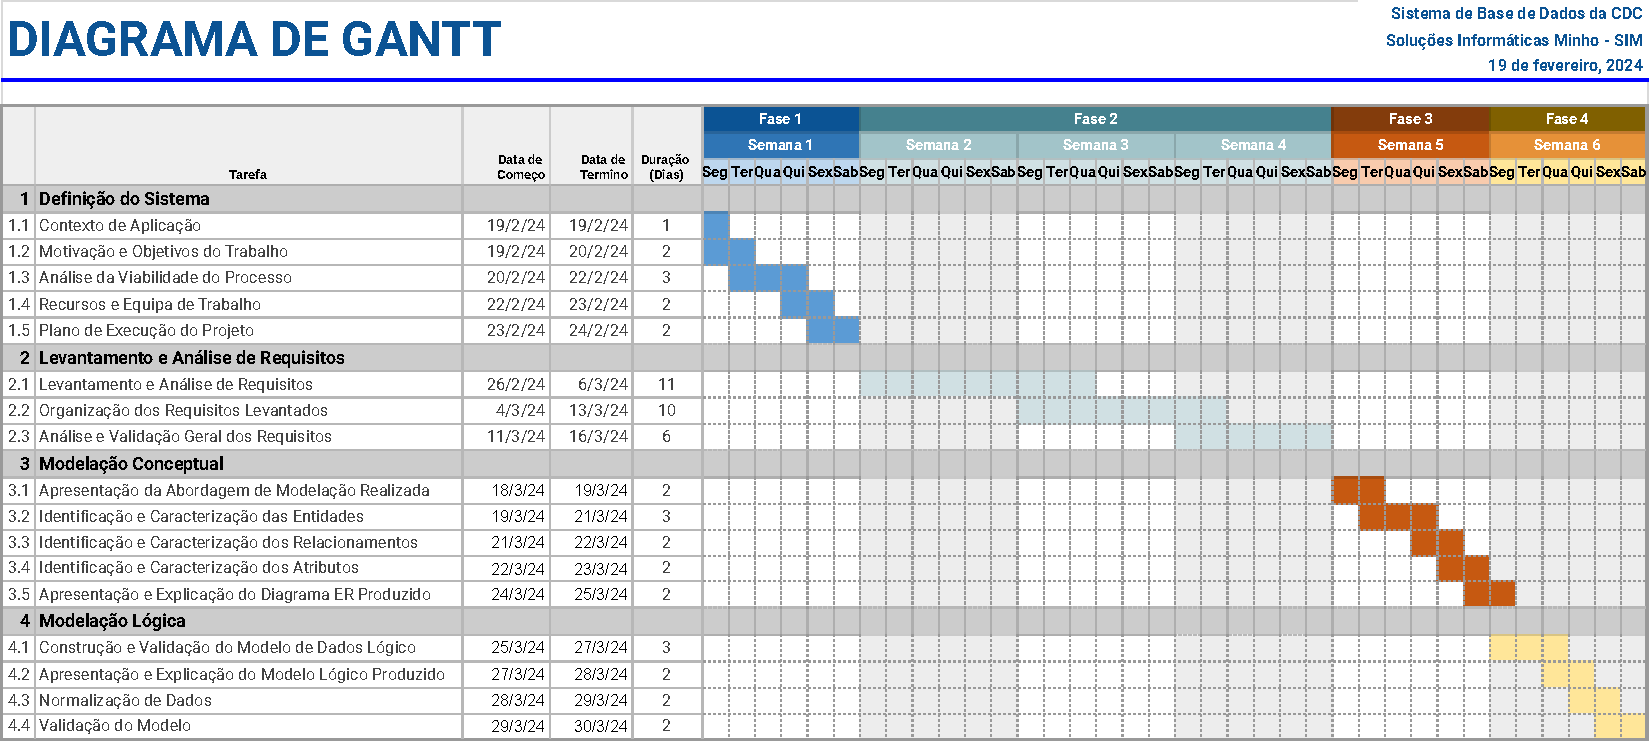
\includegraphics[scale=0.99, angle=270]{images/gantt1.pdf}
            \caption{Diagrama de Gantt - Primeira Fase}
            \label{fig:1.1}
        \end{figure}

        \begin{figure}
            \centering
            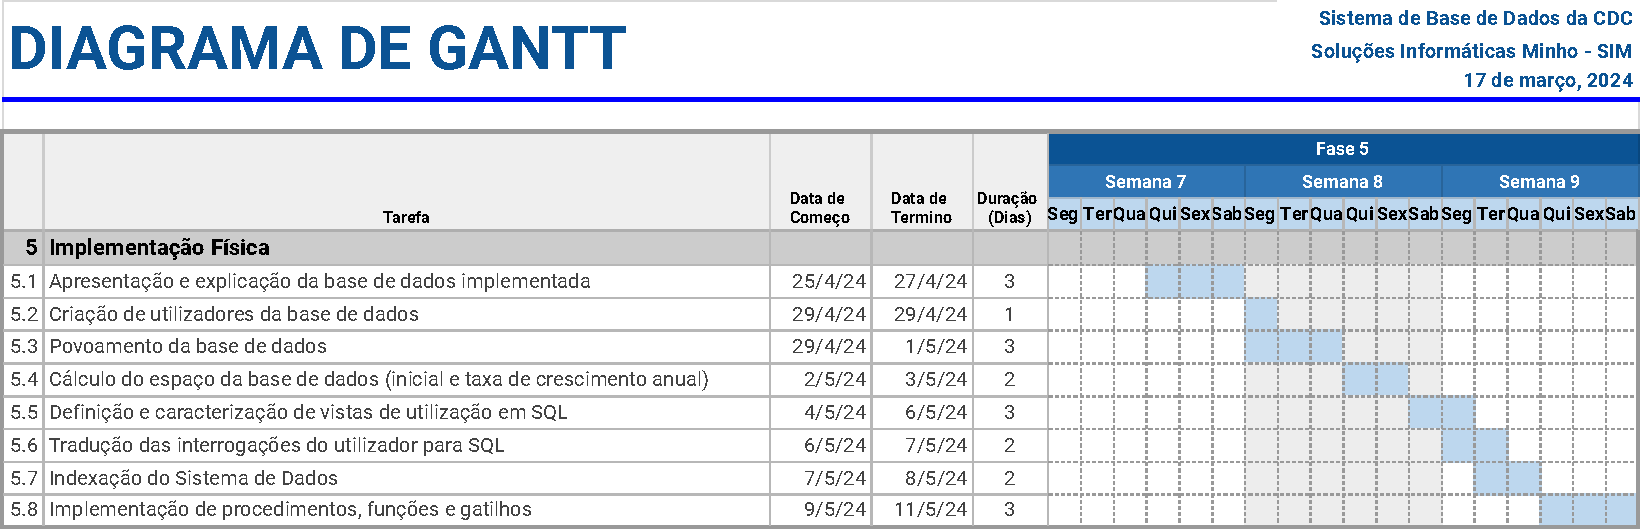
\includegraphics[scale=0.99, angle=270]{images/gantt2.pdf}
            \caption{Diagrama de Gantt - Segunda Fase}
            \label{fig:1.2}
        \end{figure}

        \loadgeometry{default}

    \clearpage
    
    \section{Estrutura do Relatório}
    O presente relatório é composto por cinco capítulos.
    
    No primeiro capítulo, \textbf{contextualizamos} o projeto que iremos desenvolver, definindo a \textbf{motivação e objetivos} por detrás deste, bem como a sua \textbf{viabilidade}. Também listamos os \textbf{recursos necessários} para a execução deste projeto, bem como o seu \textbf{planeamento}, fazendo uma análise das várias etapas deste trabalho.

    No segundo capítulo, descrevemos o \textbf{método de levantamento e de análise de requisitos adotado}, detalhando as estratégias de levantamento, organização e categorização de requisitos. Seguidamente, apresentamos os requisitos organizados por \textbf{requisitos de descrição}, de \textbf{manipulação} e de \textbf{controlo}. Por fim, \textbf{validamos} todos os requisitos levantados.

    No capítulo três, introduzimos a \textbf{modelação conceptual} desenvolvida, começando pela \textbf{identificação e caracterização das entidades}, \textbf{dos relacionamentos} e \textbf{dos atributos das entidades e dos relacionamentos} do modelo. Posto isto, é feita uma \textbf{apresentação do diagrama ER produzido}, bem como uma explicação do processo de construção do mesmo.

    No capítulo quatro, apresentamos a \textbf{modelação lógica} desenvolvida através do modelo conceptual. Aprofundamos o seu processo de \textbf{construção e validação}, e, após realizarmos o processo de conversão, apresentamos e explicamos o \textbf{modelo lógico produzido}.
    Por fim, e ainda no quarto capítulo, entramos em detalhe sobre a \textbf{normalização de dados} e \textbf{validação do modelo com interrogações do utilizador}, utilizando álgebra relacional para exemplos de acesso a dados.

    No capítulo cinco, começamos o processo de \textbf{implementação física}, onde detalhamos a execução concreta do modelo lógico na forma de uma BD. Começamos com a \textbf{apresentação e explicação da base de dados implementada}, descrevendo a estrutura das tabelas, relações entre elas e as restrições de integridade definidas. Seguidamente, abordamos a \textbf{criação de utilizadores da base de dados}, destacando os diferentes privilégios atribuídos a cada utilizador de acordo com as necessidades do sistema.
    O \textbf{povoamento da base de dados} é então discutido, onde descrevemos o processo de inserção inicial de dados na base de dados, seja por meio de um \textit{script} de SQL ou através de um programa em \textit{Python}.
    É também realizada uma análise sobre o \textbf{cálculo do espaço da base de dados}, de forma a garantir uma gestão eficiente dos recursos de armazenamento.
    De seguida, a \textbf{definição e caracterização de vistas de utilização em SQL} são apresentadas, bem como a  \textbf{tradução das interrogações do utilizador para SQL}, de forma a moldar a BD de acordo com os requisitos definidos previamente.
    A \textbf{indexação do sistema de dados} é também implementada neste capítulo, como parte crucial da otimização do desempenho da base de dados.
    Por fim, é abordada a \textbf{implementação de procedimentos, funções e gatilhos}, algo que foi essencial para melhorar a
    eficiência, a integridade e a automatização da BD.

Com este capítulo, concluímos a implementação prática do projeto, fornecendo uma base sólida para a sua utilização e manutenção contínua.

%==========================================================================
% END INTRODUCTION
%==========================================================================

%==========================================================================
% BEGIN LEVANTAMENTO E ANÁLISE DE REQUISITOS
%==========================================================================

\chapter{Levantamento e Análise de Requisitos}
    \label{sec:requisitos}
    \section{Método de Levantamento e de Análise de Requisitos Adotado}
        \label{sec:2.1}
            O processo de definição de requisitos começa com uma reunião com a equipa para selecionar diversas estratégias de levantamento, de modo a captar toda a informação necessária para sustentar adequadamente e logicamente uma melhor esquematização e composição de requisitos. Das várias estratégias discutidas, assumimos que utilizamos estas:
            \begin{itemize}
            \item \textbf{Reuniões} presenciais ou em regime \textit{online} com a Sra$.$ Christie e os seus Detetives, tanto em grupo quanto individualmente com o propósito de identificar os diversos processos operacionais que ocorrem na consultoria e classificá-los.
            \item \textit{\textbf{Emails}}, às vezes as melhores ideias podem surgir subitamente, e como os funcionários têm uma vida bastante atarefada, deste modo podemos comunicar de maneira mais ágil.
            \item \textbf{Análise de Documentação} como \textbf{artigos de jornais} sobre casos resolvidos pela consultoria, para a equipa estar mais contextualizada acerca da mesma.
            \textbf{Relatórios de casos resolvidos} são recursos escassos infelizmente, pelo que também recorremos à \textbf{leitura de entrevistas dos detetives} para uma melhor compreensão das estratégias e métodos que estes têm por hábito utilizar na sua resolução dos seus casos. Analisámos igualmente a \textbf{documentação} da própria consultoria, mais especificamente relatórios relacionados com os ganhos e custos ao longo dos anos da empresa.
            \end{itemize}
            
            Durante a reunião foi levantada a possibilidade de acompanhar uma investigação de perto, infelizmente foi negada por questões de segurança e de confidencialidade das informações dos participantes da investigação. 

    \section{Organização dos Requisitos Levantados}
        \label{sec:2.2}
        \subsection{Requisitos de Descrição}
        Os seguintes requisitos de descrição foram provenientes de reuniões com Agatha Christie e a sua Consultoria, onde foram definidos os dados que cada entidade deve possuir, bem como os relacionamentos entre si.

        \newgeometry{top=2cm,left=2cm,right=2cm,bottom=3cm}

            \begin{table}[!ht]
                \centering
                \renewcommand{\arraystretch}{1.3}
                
                \begin{tabular}{|p{0.3cm}|p{4cm}|p{3cm}|p{4.5cm}|p{3cm}|}
                \Header{green!20!white}

                1 & \multicolumn{4}{c|}{\pbox{15cm}{Cada caso tem um identificador único, representado por um número inteiro, numerado sequencialmente.}}\\
                \cline{2-5}
                & 2024/03/20 18:05:00 & Casos & Equipa de Projeto & Miguel Carvalho \\
                \hline
                
                2 & \multicolumn{4}{c|}{\pbox{15cm}{Um registo de um caso deve incluir os seguintes atributos: identificador único, identificador de cliente, identificador (número inteiro) do estado, categoria, descrição, data de abertura, data de fechamento (opcional), um atributo composto multivalorado “pagamentos” - constituído por valor, descrição e data -, e um atributo composto multivalorado “despesas” - constituído por valor, descrição e data.}}\\
                \cline{2-5}
                & 2024/03/20 18:05:00 & Casos & Equipa de Projeto & Miguel Carvalho \\
                \hline

                3 & \multicolumn{4}{c|}{\pbox{15cm}{O atributo “estado” de um caso é mapeado por um dos seguintes valores: 1 (“aberto”), 2 (“resolvido”) ou 3 (“arquivado”).}}\\
                \cline{2-5}
                & 2024/03/10 09:20:00 & Casos & Gerência & Miguel Carvalho\\
                \hline

                4 & \multicolumn{4}{c|}{\pbox{15cm}{O atributo “categoria” de um caso é mapeado por um dos seguintes valores: 1 (“Criminal”), 2 (“Civil”), 3 (“Financeiro”), 4 (“Cibernético”), 5 (“Laboral”), 6 (“Administrativo”) ou 7 (“Ético”).}}\\
                \cline{2-5}
                & 2024/03/25 21:40:00 & Casos & Gerência & Miguel Carvalho \\
                \hline

                6 & \multicolumn{4}{c|}{\pbox{15cm}{Todos os casos abertos têm vinculados pelo menos um detetive.}}\\
                \cline{2-5}
                & 2024/03/20 18:25:00 & Casos & Equipa de Projeto & Flávia Araújo\\
                \hline

                7 & \multicolumn{4}{c|}{\pbox{15cm}{Todos os casos têm associado um único cliente.}}\\
                \cline{2-5}
                & 20/03/2024 18:25 & Casos & Equipa de Projeto & Miguel Carvalho\\
                \hline

                8 & \multicolumn{4}{c|}{\pbox{15cm}{Todos os casos têm zero ou mais testemunhas.}}\\
                \cline{2-5}
                & 20/03/2024 18:25 & Casos & Equipa de Projeto & Flávia Araújo\\
                \hline

                9 & \multicolumn{4}{c|}{\pbox{15cm}{Todos os casos têm zero ou mais suspeitos.}}\\
                \cline{2-5}
                & 20/03/2024 18:25 & Casos & Equipa de Projeto & Flávia Araújo\\
                \hline

                10 & \multicolumn{4}{c|}{\pbox{15cm}{Todos os casos têm zero ou mais evidências.}}\\
                \cline{2-5}
                & 20/03/2024 18:25 & Casos & Equipa de Projeto & Miguel Carvalho\\
                \hline
                
                14 & \multicolumn{4}{c|}{\pbox{15cm}{Cada detetive tem um identificador único, representado por um número inteiro, numerado sequencialmente.}}\\
                \cline{2-5}
                & 20/03/2024 18:40 & Detetives & Equipa de Projeto & Flávia Araújo\\
                \hline
                
                15 & \multicolumn{4}{c|}{\pbox{15cm}{Um registo de um detetive deve incluir os seguintes atributos: identificador único, nome completo, telefone (único), email (único), data de nascimento, endereço de morada (opcional), salário, data de contratação, data de fim de contrato (opcional), área de especialidade, efetivo (valor booleano) e estado.}}\\
                \cline{2-5}
                & 10/03/2024 10:20 & Detetives & Equipa de Projeto & Miguel Carvalho\\
                \hline

                \end{tabular}
            \caption{Requisitos de Descrição I}
        \end{table}

            \begin{table}[!ht]
                \centering
                \renewcommand{\arraystretch}{1.3}
                \begin{tabular}{|p{0.3cm}|p{4cm}|p{3cm}|p{4.5cm}|p{3cm}|}
                \Header{green!20!white}

                16 & \multicolumn{4}{c|}{\pbox{15cm}{O atributo “área de especialidade” de um detetive é mapeado por um dos seguinte valores: 1 (“Investigação e descoberta de esquemas de fraude”), 2 (“Investigações de natureza jurídica”), 3 (“Busca e apreensão”), 4 (“Serviços corporativos”), 5 (“Aplicativo espião sobre identidades particulares”), 6 (“Aplicativo espião sobre identidades cooperativas”), 7 (“Detetive particular criminalista”) ou 8 (“Investigações cibernéticas”).}}\\
                \cline{2-5}
                & 20/03/2024 18:25 & Detetives & Equipa de Projeto & Miguel Carvalho\\
                \hline

                17 & \multicolumn{4}{c|}{\pbox{15cm}{O atributo “estado” de um detetive é mapeado por um dos seguintes valores: 1 (“contratado”), 2 (“demitido”) ou 3 (“aposentado”).}}\\
                \cline{2-5}
                & 10/03/2024 10:42 & Detetives & Equipa de Projeto & Miguel Carvalho\\
                \hline

                18 & \multicolumn{4}{c|}{\pbox{15cm}{Todos os detetives têm vinculado zero ou mais casos.}}\\
                \cline{2-5}
                & 20/03/2024 18:25 & Detetives & Equipa de Projeto & Flávia Araújo\\
                \hline

                22 & \multicolumn{4}{c|}{\pbox{15cm}{Cada cliente tem um identificador único, representado por um número inteiro, numerado sequencialmente.}}\\
                \cline{2-5}
                & 10/03/2024 12:38 & Clientes & Equipa de Projeto & Miguel Carvalho\\
                \hline

                23 & \multicolumn{4}{c|}{\pbox{15cm}{Um registo de um cliente deve incluir os seguintes atributos: identificador único, nome completo, telefone, email (opcional), e endereço de morada (opcional).}}\\
                \cline{2-5}
                & 10/03/2024 12:37 & Clientes & Equipa de Projeto & Miguel Carvalho\\
                \hline

                24 & \multicolumn{4}{c|}{\pbox{15cm}{Todos os clientes têm um ou mais casos associados.}}\\
                \cline{2-5}
                & 10/03/2024 12:39 & Clientes & Equipa de Projeto & Miguel Carvalho\\
                \hline

                25 & \multicolumn{4}{c|}{\pbox{15cm}{Cada testemunha tem um identificador único, representado por um número inteiro, numerado sequencialmente.}}\\
                \cline{2-5}
                & 10/03/2024 12:39 & Testemunhas & Equipa de Projeto & Miguel Carvalho\\
                \hline

                26 & \multicolumn{4}{c|}{\pbox{15cm}{Um registo de uma testemunha deve incluir os seguintes atributos: identificador único, nome completo, telefone (único), email (único), endereço de morada (opcional) e data de registo.}}\\
                \cline{2-5}
                & 10/03/2024 11:00 & Testemunhas & Equipa de Projeto & Miguel Carvalho\\
                \hline

                27 & \multicolumn{4}{c|}{\pbox{15cm}{Devido a natureza do relacionamento entre testemunhas e casos (N:M) é feito um mapeamento entre os identificadores de caso e de testemunha.}}\\
                \cline{2-5}
                & 10/03/2024 13:20 & Testemunhas & Equipa de Projeto & Miguel Carvalho\\
                \hline

                28 & \multicolumn{4}{c|}{\pbox{15cm}{Cada suspeito tem um identificador único, representado por um número inteiro, numerado sequencialmente.}}\\
                \cline{2-5}
                & 10/03/2024 12:40 & Suspeitos & Equipa de Projeto & Miguel Carvalho\\
                \hline

                29 & \multicolumn{4}{c|}{\pbox{15cm}{Um registo de um suspeito deve incluir os seguintes atributos: identificador único, nome completo, telefone (opcional), email (opcional), data de nascimento (opcional), sexo (opcional), endereço de morada (opcional), descrição (opcional) e data de registo.}}\\
                \cline{2-5}
                & 10/03/2024 11:01 & Suspeitos & Equipa de Projeto & Miguel Carvalho\\
                \hline

                30 & \multicolumn{4}{c|}{\pbox{15cm}{O atributo “descrição” de um suspeito contém informações sobre o mesmo, desde o porquê da suspeita, histórico criminal, etc.}}\\
                \cline{2-5}
                & 25/03/2024 21:45 & Suspeitos & Funcionários & Miguel Carvalho\\
                \hline

                31 & \multicolumn{4}{c|}{\pbox{15cm}{Devido a natureza do relacionamento entre suspeitos e casos (N:M) é feito um mapeamento entre os identificadores de caso e de suspeito.}}\\
                \cline{2-5}
                & 10/03/2024 13:25 & Suspeitos & Equipa de Projeto & Miguel Carvalho\\
                \hline

                \end{tabular}
            \caption{Requisitos de Descrição II}
        \end{table}

            \begin{table}[!ht]
                \centering
                \renewcommand{\arraystretch}{1.3}
                \begin{tabular}{|p{0.3cm}|p{4cm}|p{3cm}|p{4.5cm}|p{3cm}|}
                \Header{green!20!white}

                32 & \multicolumn{4}{c|}{\pbox{15cm}{Um registo de uma vinculação efetua a ligação entre um caso e os seus detetives, e deve incluir os seguintes atributos: data de vinculação, data de desvinculação (opcional) e descrição.}}\\
                \cline{2-5}
                & 10/03/2024 12:30 & Vinculações & Gerência & Miguel Carvalho\\
                \hline

                34 & \multicolumn{4}{c|}{\pbox{15cm}{Cada evidência tem um identificador único, representado por um número inteiro, numerado sequencialmente.}}\\
                \cline{2-5}
                & 10/03/2024 12:50 & Evidências & Equipa de Projeto & Miguel Carvalho\\
                \hline

                35 & \multicolumn{4}{c|}{\pbox{15cm}{Um registo de uma evidência deve incluir os seguintes atributos: identificador único, identificador do caso, data de coleta, descrição, tipo e arquivo (opcional).}}\\
                \cline{2-5}
                & 10/03/2024 12:50 & Evidências & Equipa de Projeto & Miguel Carvalho\\
                \hline

                36 & \multicolumn{4}{c|}{\pbox{15cm}{O atributo “tipo” de uma evidência é mapeado por um dos seguintes valores: 1 (“testemunhal”), 2 (“documental”), 3 (“pericial”), 4 (“indicial”) ou 5 (“real”).}}\\
                \cline{2-5}
                & 10/03/2024 12:57 & Evidências & Funcionários & Miguel Carvalho\\
                \hline

                37 & \multicolumn{4}{c|}{\pbox{15cm}{O atributo “arquivo” de uma evidência representa a localização de um ficheiro digital ou um link, podendo este ser uma foto, vídeo, áudio ou documento.}}\\
                \cline{2-5}
                & 10/03/2024 12:59 & Evidências & Funcionários & Miguel Carvalho\\
                \hline

                38 & \multicolumn{4}{c|}{\pbox{15cm}{Todos as evidências têm associadas um único caso.}}\\
                \cline{2-5}
                & 25/03/2024 21:45 & Evidências & Equipa de Projeto & Miguel Carvalho\\
                \hline

                \end{tabular}
            \caption{Requisitos de Descrição III}
        \end{table}

        \clearpage

        \loadgeometry{default}

         \subsection{Requisitos de Manipulação}
         Os requisitos de manipulação apresentados foram desenvolvidos após reuniões e consulta dos registos físicos da Consultoria, que, tal como referido anteriormente, causavam dificuldades na procura de informação.
         
         Para tal, foram desenvolvidos os requisitos \textbf{11, 13, 19 e 21} para uma melhor organização dos dados e um acesso mais eficiente aos mesmos.
         
         Foram também desenvolvidos os requisitos \textbf{5, 12, 19, 20 e 33} para uma melhor gestão de funcionários, de forma a saber quem está a trabalhar em casos de momento.

         Os requisitos \textbf{44} a \textbf{48} foram desenvolvidos com o propósito de resolver confusões financeiras que os registos antigos causavam e agilizar o processo de faturação.

         Por fim, os requisitos \textbf{49, 50 e 51} geram relatórios pedidos por Agatha Christie tanto a nível de despesas e pagamentos, bem como de informações sobre os casos.

         \newgeometry{top=2cm,left=2cm,right=2cm,bottom=3cm}

            \begin{table}[!ht]
                \centering
                \renewcommand{\arraystretch}{1.3}
                \begin{tabular}{|p{0.3cm}|p{4cm}|p{3cm}|p{4.5cm}|p{3cm}|}
                \Header{blue!20!white}

                5 & \multicolumn{4}{c|}{\pbox{15cm}{Quando um caso é resolvido ou arquivado o seu estado é atualizado respetivamente, assim como a data de fechamento e é feita a desvinculação dos seus detetives.}}\\
                \cline{2-5}
                & 10/03/2024 09:22 & Casos & Gerência & Miguel Carvalho\\
                \hline

                11 & \multicolumn{4}{c|}{\pbox{15cm}{Os dados relativos de cada caso - evidências, suspeitos e testemunhas - devem ser apresentados por ordem cronológica.}}\\
                \cline{2-5}
                & 20/03/2024 18:07 & Casos & Funcionários & Miguel Carvalho\\
                \hline

                12 & \multicolumn{4}{c|}{\pbox{15cm}{Dado o identificador do caso, deve ser possível aceder a todos os detetives que já estiveram envolvidos, bem como detetives envolvidos no momento.}}\\
                \cline{2-5}
                & 12/03/2024 19:40 & Casos & Gerência & Miguel Carvalho\\
                \hline

                13 & \multicolumn{4}{c|}{\pbox{15cm}{O sistema permite a pesquisa de características comuns entre casos, através da pesquisa de descrições nas seguintes entidades: casos, evidências e suspeitos.}}\\
                \cline{2-5}
                & 25/03/2024 21:50 & Casos & Funcionários & Miguel Carvalho\\
                \hline

                19 & \multicolumn{4}{c|}{\pbox{15cm}{Dado o identificador de um detetive, deve ser possível aceder a todos os casos em que esteve/está envolvido.}}\\
                \cline{2-5}
                & 20/03/2024 18:35 & Detetives & Gerência & Miguel Carvalho\\
                \hline

                20 & \multicolumn{4}{c|}{\pbox{15cm}{Quando um detetive é demitido ou se aposenta o seu atributo “estado” deve ser atualizado respetivamente, assim como o atributo “data de desvinculação” de todas as suas vinculações a casos.}}\\
                \cline{2-5}
                & 10/03/2024 13:10 & Detetives & Gerência & Miguel Carvalho\\
                \hline

                21 & \multicolumn{4}{c|}{\pbox{15cm}{Os dados relativos a um detetive devem ser acedidos através do seu identificador único.}}\\
                \cline{2-5}
                & 20/03/2024 18:30 & Detetives & Equipa de Projeto & Miguel Carvalho\\
                \hline

                33 & \multicolumn{4}{c|}{\pbox{15cm}{Uma desvinculação de um detetive a um caso, sejam os motivos aposentamento/demissão/remoção do detetive, deve atualizar o atributo “data de desvinculação”.}}\\
                \cline{2-5}
                & 10/03/2024 12:35 & Vinculações & Gerência & Miguel Carvalho\\
                \hline

                \end{tabular}
            \caption{Requisitos de Manipulação I}
        \end{table}

            \begin{table}[!ht]
                \centering
                \renewcommand{\arraystretch}{1.3}
                \begin{tabular}{|p{0.3cm}|p{4cm}|p{3cm}|p{4.5cm}|p{3cm}|}
                \Header{blue!20!white}

                44 & \multicolumn{4}{c|}{\pbox{15cm}{É permitido pelo sistema obter o custo total de um caso, através da soma de todas as despesas relativas ao mesmo. Salários de detetives não estão incluídos.}}\\
                \cline{2-5}
                & 10/03/2024 16:25 & Financeiro & Gerência & Miguel Carvalho\\
                \hline

                45 & \multicolumn{4}{c|}{\pbox{15cm}{É permitido pelo sistema obter o rendimento total de um caso, através da soma de todos os pagamentos relativos ao mesmo.}}\\
                \cline{2-5}
                & 10/03/2024 16:25 & Financeiro & Gerência & Miguel Carvalho\\
                \hline

                46 & \multicolumn{4}{c|}{\pbox{15cm}{É permitido pelo sistema obter o lucro/prejuízo de um caso, através da subtração do valor obtido em \textbf{R45} (rendimento) pelo valor obtido em \textbf{R44} (custo).}}\\
                \cline{2-5}
                & 10/03/2024 16:26 & Financeiro & Gerência & Miguel Carvalho\\
                \hline

                47 & \multicolumn{4}{c|}{\pbox{15cm}{É permitido pelo sistema obter todas as despesas efetuadas por um detetive em diferentes casos em que este participou.}}\\
                \cline{2-5}
                & 10/03/2024 16:40 & Financeiro & Gerência & Miguel Carvalho\\
                \hline

                48 & \multicolumn{4}{c|}{\pbox{15cm}{É permitido pelo sistema obter todos os pagamentos efetuados por um cliente em diferentes casos.}}\\
                \cline{2-5}
                & 10/03/2024 16:50 & Financeiro & Gerência & Miguel Carvalho\\
                \hline

                49 & \multicolumn{4}{c|}{\pbox{15cm}{No encerramento de cada dia, o sistema deverá gerar um relatório que inclua todas as despesas e pagamentos efetuados. Este deve apresentar individualmente cada despesa e pagamento, se existirem, por caso. Adicionalmente, o relatório deve fornecer o somatório total de despesas, pagamentos, bem como os lucros ou prejuízos acumulados nesse dia.}}\\
                \cline{2-5}
                & 11/03/2024 19:40 & Financeiro & Gerência & Miguel Carvalho\\
                \hline

                50 & \multicolumn{4}{c|}{\pbox{15cm}{No encerramento de cada dia, o sistema deverá gerar um relatório para cada caso que inclua novas evidências, testemunhas e suspeitos.}}\\
                \cline{2-5}
                & 20/03/2024 18:40 & Casos & Gerência & Miguel Carvalho\\
                \hline

                51 & \multicolumn{4}{c|}{\pbox{15cm}{No encerramento de cada semana, o sistema deverá gerar um relatório com informações e estatísticas relativas a novos casos abertos, fechados e/ou arquivados.}}\\
                \cline{2-5}
                & 20/03/2024 18:40 & Casos & Gerência & Miguel Carvalho\\
                \hline

                \end{tabular}
            \caption{Requisitos de Manipulação II}
        \end{table}
        \clearpage

         \subsection{Requisitos de Controlo}  
         Os requisitos de controlo desenvolvidos foram planeados tendo em conta as permissões de acesso que Agatha Christie pretendia ter na sua Consultoria. Como tal, o requisito \textbf{41} refere-se às permissões de um detetive estagiário, os requisitos \textbf{40} e \textbf{42} referem-se às permissões dos detetives envolvidos nos casos de momento, e o requisito \textbf{43} refere-se às permissões de administrador da BD (Agatha Christie). 

         
            \begin{table}[!ht]
                \centering
                \renewcommand{\arraystretch}{1.3}
                \begin{tabular}{|p{0.3cm}|p{4cm}|p{3cm}|p{4.5cm}|p{3cm}|}
                \Header{red!20!white}

                39 & \multicolumn{4}{c|}{\pbox{15cm}{O sistema deve estar operacional durante 24 horas por dia, 7 dias por semana, sem interrupções.}}\\
                \cline{2-5}
                & 11/03/2024 20:10 & Sistema & Equipa de Projeto & Miguel Carvalho\\
                \hline

                40 & \multicolumn{4}{c|}{\pbox{15cm}{O sistema deve garantir que apenas os detetives que estão vinculados a um determinado caso, podem alterar os dados relativos ao mesmo.}}\\
                \cline{2-5}
                & 10/03/2024 11:20 & Permissões & Gerência & Miguel Carvalho\\
                \hline

                41 & \multicolumn{4}{c|}{\pbox{15cm}{O sistema deve garantir que os detetives estagiários apenas podem ler dados relativos a casos não abertos, ou seja, casos fechados e arquivados.}}\\
                \cline{2-5}
                & 20/03/2024 18:35 & Permissões & Gerência & Miguel Carvalho\\
                \hline

                42 & \multicolumn{4}{c|}{\pbox{15cm}{O sistema deve oferecer acesso aos dados de um caso aberto apenas aos detetives a si associados e a Agatha Christie.}}\\
                \cline{2-5}
                & 11/03/2024 20:02 & Permissões & Gerência & Miguel Carvalho\\
                \hline

                43 & \multicolumn{4}{c|}{\pbox{15cm}{Os administradores devem ser capazes de ler, adicionar, atualizar e remover as informações armazenadas na base de dados.}}\\
                \cline{2-5}
                & 11/03/2024 20:05 & Permissões & Equipa de Projeto & Miguel Carvalho\\
                \hline

                \end{tabular}
            \caption{Requisitos de Controlo I}
        \end{table}

        \loadgeometry{default}

        \textbf{Nota}: Consultar anexo \textit{\nameref{anexo:2}} para a visualização do Documento Geral de Recolha, bem como os documentos de Requisitos de Descrição, Requisitos de Manipulação e Requisitos de Controlo originais.
        
    \section{Análise e Validação Geral dos Requisitos}
        
        Após o levantamento e a recolha dos requisitos através dos métodos apresentados no subcapítulo [\ref{sec:2.1}] do presente relatório, foi necessário fazer a qualificação dos mesmos. Para isso, o pessoal externo da equipa de trabalho procedeu à separação dos requisitos recolhidos nas três categorias apresentadas no subcapítulo [\ref{sec:2.2}].
        
        Numa última fase, a equipa de trabalho, não podendo prosseguir o desenvolvimento do projeto sem a revisão, por parte do cliente, dos requisitos já tratados, reuniu com a gerente da empresa, Agatha Christie. Esta, por sua vez, fez alguns reparos a alguns requisitos, que prontamente, em coordenação com a equipa de trabalho, foram reajustados. Por fim, foi aprovada a lista final de requisitos podendo, assim, o projeto entrar numa nova fase de desenvolvimento.

%==========================================================================
% END LEVANTAMENTO E ANÁLISE DE REQUISITOS
%==========================================================================

%==========================================================================
% BEGIN MODELAÇÃO CONCEPTUAL
%==========================================================================

\chapter{Modelação Conceptual}
    \section{Apresentação da Abordagem de Modelação Realizada}
        {
            Após o levantamento dos requisitos com a informação obtida, iniciámos o processo de planeamento da estrutura do Sistema de Gestão de Bases de Dados que almejamos implementar.
            Posto isto, começámos pela modelação conceptual do nosso projeto através da construção de um Diagrama ER, de modo a podermos visualizar como as entidades (caso, detetive, cliente, etc.) relacionar-se-iam entre si, bem como os atributos que ambos (entidades e relacionamentos) possam ter. Para a caracterização das entidades, atributos e relacionamentos nos subcapítulos seguintes, recorremos à caracterização sugerida em  \cite{DatabaseSystems} (Connolly \& Begg, 2015).

            Para a construção do diagrama em si, recorremos à ferramenta BR Modelo, que utiliza notação baseada na de Dr$.$ Heuser (sendo esta fortemente alicerçada na notação de Peter Chen, como consultado em \cite{Aprendizagem em Banco de Dados} (Cândido, 2005)).
        }

    \clearpage
        
    \section{Identificação e Caracterização das Entidades}
        Avaliando o funcionamento da agência de detetives de Agatha, concluímos que as entidades seriam caracterizadas pelo conjunto: Caso, Detetive, Evidência, Cliente, Suspeito e Testemunha.

        Para cumprir os requisitos levantados anteriormente, estas entidades possuem os seguintes atributos:

        \begin{itemize}
        \item \textbf{Caso:} Representa cada caso registado na agência, trazido por um cliente e investigado por detetives.
            \begin{itemize}
            \item\textbf{Sinónimos:} Investigação, Processo, Arquivo. 
            \item\textbf{Atributos:} ID, Descrição, Estado, Categoria, Data de Abertura, Data de Fechamento, Despesa (multivalorado, com Valor, Data e Descrição) e Pagamento (também multivalorado, com Valor, Data e Descrição).
            \end{itemize}

        \item \textbf{Detetive:} Representa cada detetive que trabalha na agência em cargo da investigação de casos.
            \begin{itemize}
            \item\textbf{Sinónimos:} Investigador, Funcionário, Agente.
            \item\textbf{Atributos:} ID, Nome, \textit{Email}, Telefone, Data de Nascimento, Morada, Salário, Data de Contratação, Data de Fim de Contratação, Efetivo, Estado e Especialidade.
            \end{itemize}

        \item \textbf{Evidência:} Representa cada evidência que os detetives encontraram sobre um caso, podendo esta ter sido fornecida por uma testemunha e/ou cliente e incriminatória a um suspeito.
            \begin{itemize}
            \item\textbf{Sinónimos:} Prova, Testemunho, Depoimento. 
            \item\textbf{Atributos:} ID, Data de Coleta, Descrição, Tipo e Arquivo.
            \end{itemize}

        \item \textbf{Cliente:} Representa cada cliente que contrata a agência com o intuito dos detetives resolverem o caso que propõe.
            \begin{itemize}
            \item\textbf{Sinónimos:} Inquirido, Consumidor.
            \item\textbf{Atributos:} ID, Nome, \textit{Email}, Telefone e Morada. 
            \end{itemize}

        \clearpage

        \item \textbf{Suspeito:} Representa cada indivíduo considerado suspeito aquando a investigação de um caso por detetives.
            \begin{itemize}
            \item\textbf{Sinónimos:} Acusado, Culpado, Réu, Arguido. 
            \item\textbf{Atributos:} ID, Nome, \textit{Email}, Telefone, Data de Nascimento, Sexo, Morada, Descrição e Data de Registo.
            \end{itemize}

        \item \textbf{Testemunha:} Representa cada testemunha que fornece informação aos detetives aquan-do a investigação de um caso.
            \begin{itemize}
            \item\textbf{Sinónimos:} Informante, Depoente, Testificador.
            \item\textbf{Atributos:} ID, Nome, \textit{Email}, Telefone, Morada e Data de Registo.
            \end{itemize}
        \end{itemize}

\pagebreak
    \section{Identificação e Caracterização dos Relacionamentos}
        \label{sec:relacionamentos}
        Na nossa modelação, englobámos cinco tipos de relacionamentos entre as entidades - três dos quais originam uma entidade. Devido a estas diferenças, aprofundaremos de forma individual cada um deles neste subcapítulo.

        \vspace{0.5cm}

        \begin{itemize}
        \item\textbf{Relacionamento Detetive-Caso}
        \begin{itemize}
            \item\textbf{Relacionamento:} Detetive vinculado a Caso.
            \item\textbf{Descrição:} Com o intuito de poder estabelecer as vinculações dos detetives aos casos, é importante armazenar a informação desta forma para saber que detetives estão vinculados a quais casos, e durante quanto tempo foi a sua vinculação a estes. Saberemos, deste modo, se um caso tem os detetives necessários e/ou se certos detetives estão livres para serem encaminhados para novos casos.
            \item\textbf{Multiplicidade:} Detetive (0,n) - Caso (0,n): Todos os detetives têm pelo menos zero ou mais casos vinculados, e todos os casos abertos têm pelo menos um detetive vinculado, porém casos arquivados ou fechados não têm detetives vinculados.
            \item\textbf{Baseado nos Requisitos:}
            \begin{itemize}
                \item [R6]: “Todos os casos abertos têm vinculados pelo menos um detetive.”
                \item [R18]: “Todos os detetives têm vinculado zero ou mais casos.”
                \item [R32]: “Um registo de uma vinculação efetua a ligação entre um caso e os seus detetives, e deve incluir os seguintes atributos: data de vinculação, data de desvinculação (opcional) e descrição.”
            \end{itemize}
            \item\textbf{Atributos:} Data de Vinculação, Data de Desvinculação e Descrição.
            \item\textbf{Entidade Gerada:} Vinculação.
        \end{itemize}
        
        %%\vspace{0.5cm}
        \clearpage

        \item\textbf{Relacionamento Evidência-Caso}
        \begin{itemize}
            \item\textbf{Relacionamento:} Evidência referente a Caso
            \item\textbf{Descrição:} Visto que evidências são fatores cruciais num caso, é importante o armazenamento das informações desta maneira de forma a poder facilmente aceder a todas as evidências encontradas referentes a um caso em específico, deste modo garante-se um acesso mais eficiente à informação desejada.
            \item\textbf{Multiplicidade:} Evidência (1,1) - Caso (0,n): Uma evidência está sempre associada a apenas um caso, e um caso pode ter zero ou mais evidências associadas.
            \item\textbf{Baseado nos Requisitos:}
            \begin{itemize}
                \item [R10]: “Todos os casos têm zero ou mais evidências.”
                \item [R38]: “Todos as evidências têm associadas um único caso.”
            \end{itemize}
            \item\textbf{Atributos:} Nenhum.
            \item\textbf{Entidade Gerada:} Nenhuma.
        \end{itemize}

        \vspace{0.75cm}

        \item\textbf{Relacionamento Cliente-Caso}
        \begin{itemize}
            \item\textbf{Relacionamento:} Cliente requisita Caso.
            \item\textbf{Descrição:} Com o intuito de poder registar que clientes requisitam quais casos, toda a informação relativa à requisição dos mesmos é armazenada desta forma.
            \item\textbf{Multiplicidade:} Cliente (1,n) - Caso (1,1): Um cliente pode estar associado a vários casos, porém um caso só pode estar associado a um cliente.
            \item\textbf{Baseado nos Requisitos:}
            \begin{itemize}
                \item [R7]: “Todos os casos têm associados um único cliente.”
                \item [R24]: “Todos os clientes têm um ou mais casos associados.”
            \end{itemize}
            \item\textbf{Atributos:} Nenhum.
            \item\textbf{Entidade Gerada:} Nenhuma.   
        \end{itemize}

        %%\vspace{0.5cm}
        \clearpage
        
        \item\textbf{Relacionamento Caso-Suspeito}
        \begin{itemize}
            \item\textbf{Relacionamento:} Caso “\textit{CasoSuspeito}” Suspeito.
            \item\textbf{Descrição:} De forma a poder registar devidamente todos os suspeitos encontrados pelos detetives relativamente a um caso que estão a investigar, é importante armazenar a informação desta forma para tal ser feito. Assim, sempre que encontrar em uma nova pista, podem voltar a rever a sua lista de suspeitos com detalhe.
            \item\textbf{Multiplicidade:} Caso (0,n) - Suspeito (1,n): Todos os casos têm zero ou mais suspeitos associados, e todos os suspeitos têm, pelo menos, um caso vinculado.
            \item\textbf{Baseado nos Requisitos:}
            \begin{itemize}
                \item [R9]: “Todos os casos têm zero ou mais suspeitos.”
                \item [R31]: “Devido a natureza do relacionamento entre suspeitos e casos (N:M) é feito um mapeamento entre os identificadores de caso e de suspeito.”
            \end{itemize}
            \item\textbf{Atributos:} Nenhum.
            \item\textbf{Entidade Gerada:} CasoSuspeito.
        \end{itemize}

        \vspace{0.75cm}
    
        \item\textbf{Relacionamento Caso-Testemunha}
        \begin{itemize}
            \item\textbf{Relacionamento:} Caso “\textit{CasoTestemunha}” Testemunha.
            \item\textbf{Descrição:} Para garantir uma investigação eficaz, é crucial documentar organizadamente todas as testemunhas encontradas relativamente a um caso, incluindo os todos os detalhes e relatos que forneceu, para referência futura e análise detalhada.
            \item\textbf{Multiplicidade:} Caso (0,n) - Testemunha (1,n): Todos os casos têm zero ou mais testemunhas associadas, e todas as testemunhas têm, pelo menos, um caso vinculado.
            \item\textbf{Baseado nos Requisitos:}
            \begin{itemize}
                \item [R8]: “Todos os casos têm zero ou mais testemunhas.”
                \item [R27]: “Devido a natureza do relacionamento entre testemunhas e casos (N:M) é feito um mapeamento entre os identificadores de caso e de testemunha.”
            \end{itemize}
            \item\textbf{Atributos:} Nenhum.
            \item\textbf{Entidade Gerada:} CasoTestemunha.
        \end{itemize}
        \end{itemize}

    \clearpage
    \section{Identificação e Caracterização dos Atributos das Entidades e dos Relacionamentos}
        
        \textbf{Entidade: \textit{Caso}}
        \begin{table}[!ht]
        \centering
        \begin{tabular}{|c|c|c|c|c|c|c|}
        \hline
        \rowcolor{gray!20!white}
        \textbf{Atributos} & \textbf{Nulo} & \textbf{Composto} & \textbf{Derivado} & \textbf{Multivalorado} & \textbf{Candidato} \\
        \hline
        ID                  & \Nao & \Nao & \Nao & \Nao & \Sim \\
        Descrição           & \Nao & \Nao & \Nao & \Nao & \Nao \\
        Estado              & \Nao & \Nao & \Nao & \Nao & \Nao \\
        Categoria           & \Nao & \Nao & \Nao & \Nao & \Nao \\
        DataAbertura        & \Nao & \Nao & \Nao & \Nao & \Nao \\
        DataFechamento      & \Sim & \Nao & \Nao & \Nao & \Nao \\
        Despesa             & \Nao & \Sim & \Nao & \Sim & \Sim \\
        Despesa.Valor       & \Nao & \Nao & \Sim & \Sim & \Nao \\
        Despesa.Data        & \Nao & \Nao & \Sim & \Sim & \Nao \\
        Despesa.Descrição   & \Nao & \Nao & \Sim & \Sim & \Nao \\
        Pagamento           & \Nao & \Sim & \Nao & \Sim & \Sim \\
        Pagamento.Valor     & \Nao & \Nao & \Sim & \Sim & \Nao \\
        Pagamento.Data      & \Nao & \Nao & \Sim & \Sim & \Nao \\
        Pagamento.Descrição & \Nao & \Nao & \Sim & \Sim & \Nao \\
        \hline
        \end{tabular}
        \caption{Identificação e Caracterização dos Atributos da Entidade \textit{Caso}}
        \end{table}

        \textbf{Caracterização dos atributos da entidade: \textit{Caso}}
        \begin{itemize}
            \item \textbf{ID}: É único e identifica cada caso existente na agência, desde abertos, resolvidos, a arquivados;
            \item \textbf{Descrição}: Um relatório acerca do caso em questão; 
            \item \textbf{Estado}: O estado do caso, isto é, se ele se encontra aberto, fechado, ou arquivado; 
            \item \textbf{Categoria}: A categoria em que o caso incide - criminal, civil, financeiro, cibernético, laboral, administrativo ou ético;
            \item \textbf{DataAbertura}: A data de abertura do caso; 
            \item \textbf{DataFechamento}: A data de encerramento do caso, se este já tiver sido fechado;

        \clearpage
            
            \item \textbf{Despesa}: A despesa relativa ao caso (salários de detetives não incluídos). Este atributo composto multivalorado é constituído por: 
            \begin{itemize}
                \item \textbf{Caso}: Identificador do caso relativo à despesa;
                \item \textbf{Valor}: Valor monetário da despesa do caso;
                \item \textbf{Data}: Data em que esta despesa foi registada;
                \item \textbf{Descrição}: Uma explanação relativa ao motivo de certa despesa.
            \end{itemize}
            \item \textbf{Pagamento}: Pagamento efetuado pelo cliente para a investigação do caso. Este atributo composto multivalorado é constituído por: 
            \begin{itemize}
                \item \textbf{Caso}: Identificador do caso relativo ao pagamento;
                \item \textbf{Valor}: Valor monetário do pagamento do cliente;
                \item \textbf{Data}: Data em que este pagamento foi registado;
                \item \textbf{Descrição}: Descrição relativa ao pagamento realizado.
            \end{itemize}
        \end{itemize}

        \clearpage
        
        \newgeometry{top=2.5cm}
        
        \textbf{Entidade: \textit{Detetive}}
        \begin{table}[!ht]
        \centering
        \begin{tabular}{|c|c|c|c|c|c|c|}
        \hline
        \rowcolor{gray!20!white}
        \textbf{Atributos} & \textbf{Nulo} & \textbf{Composto} & \textbf{Derivado} & \textbf{Multivalorado} & \textbf{Candidato} \\
        \hline
        ID                 & \Nao & \Nao & \Nao & \Nao & \Sim \\
        Nome               & \Nao & \Nao & \Nao & \Nao & \Nao \\
        Email              & \Nao & \Nao & \Nao & \Nao & \Sim \\
        Telefone           & \Nao & \Nao & \Nao & \Nao & \Sim \\
        DataNascimento     & \Nao & \Nao & \Nao & \Nao & \Nao \\
        Morada             & \Sim & \Nao & \Nao & \Nao & \Nao \\
        Salário            & \Nao & \Nao & \Nao & \Nao & \Nao \\
        DataContratação    & \Nao & \Nao & \Nao & \Nao & \Nao \\
        DataFimContratação & \Sim & \Nao & \Nao & \Nao & \Nao \\
        Efetivo            & \Nao & \Nao & \Nao & \Nao & \Nao \\
        Estado             & \Nao & \Nao & \Nao & \Nao & \Nao \\
        Especialidade      & \Nao & \Nao & \Nao & \Nao & \Nao \\
        \hline
        \end{tabular}
        \caption{Identificação e Caracterização dos Atributos da Entidade \textit{Detetive}}
        \end{table}

        \textbf{Caracterização dos atributos da entidade: \textit{Detetive}}
        \begin{itemize}
            \item \textbf{ID}: É único e identifica cada detetive existente na agência - tanto contratados, como demitidos e aposentados;
            \item \textbf{Nome}: O nome do detetive;
            \item \textbf{\textit{Email}}: O endereço de \textit{email} do detetive;
            \item \textbf{Telefone}: O número de telefone do detetive;
            \item \textbf{DataNascimento}: A data de nascimento do detetive;
            \item \textbf{Morada}: A morada do detetive;
            \item \textbf{Salário}: O salário do detetive, em euros;
            \item \textbf{DataContratação}: A data de contratação do detetive;
            \item \textbf{DataFimContratação}: A data de fim de contratação do detetive, caso ele seja demitido ou aposentado;
            \item \textbf{Efetivo}: Representa se o detetive é efetivo ou estagiário;
            \item \textbf{Estado}: O estado de um detetive, que pode ser contratado, demitido ou aposentado;
            \item \textbf{Especialidade}: A especialidade do detetive, que pode ser: Investigação e descoberta de esquemas de fraude, Investigações de natureza jurídica, Busca e apreensão, Serviços corporativos, Aplicativo espião sobre identidades particulares, Aplicativo espião sobre identidades corporativas, Detetive particular criminalista ou Investigações cibernéticas. 
        \end{itemize}

        \loadgeometry{default}

        \pagebreak
        \textbf{Entidade: \textit{Suspeito}}
        \begin{table}[!ht]
        \centering
        \begin{tabular}{|c|c|c|c|c|c|c|}
        \hline
        \rowcolor{gray!20!white}
        \textbf{Atributos} & \textbf{Nulo} & \textbf{Composto} & \textbf{Derivado} & \textbf{Multivalorado} & \textbf{Candidato} \\
        \hline
        ID                  & \Nao & \Nao & \Nao & \Nao & \Sim \\
        Nome                & \Nao & \Nao & \Nao & \Nao & \Nao \\  
        Email               & \Sim & \Nao & \Nao & \Nao & \Nao \\
        Telefone            & \Sim & \Nao & \Nao & \Nao & \Nao \\
        DataNascimento      & \Sim & \Nao & \Nao & \Nao & \Nao \\
        Sexo                & \Sim & \Nao & \Nao & \Nao & \Nao \\
        Morada              & \Sim & \Nao & \Nao & \Nao & \Nao \\
        Descrição           & \Sim & \Nao & \Nao & \Nao & \Nao \\
        DataRegisto         & \Nao & \Nao & \Nao & \Nao & \Nao \\
        \hline
        \end{tabular}
        \caption{Identificação e Caracterização dos Atributos da Entidade \textit{Suspeito}}
        \end{table}

        \textbf{Caracterização dos atributos da entidade: \textit{Suspeito}}
        \begin{itemize}
            \item \textbf{ID}: É único e identifica cada suspeito alguma vez registado na agência;
            \item \textbf{Nome}: Nome do suspeito;
            \item \textbf{\textit{Email}}: Endereço de \textit{email} do suspeito;
            \item \textbf{Telefone}: Número de telefone do suspeito;
            \item \textbf{DataNascimento}: Data de nascimento do suspeito;
            \item \textbf{Sexo}: Género do suspeito;
            \item \textbf{Morada}: Morada do suspeito;
            \item \textbf{Descrição}: Descrição do suspeito, isto é, daquilo que o torna um suspeito no caso a ser investigado e/ou o seu histórico criminal;
            \item \textbf{DataRegisto}: Data de registo do suspeito.
        \end{itemize}

        \clearpage
    \newgeometry{top=2cm}
        
        \textbf{Entidade: \textit{Testemunha}}
        \begin{table}[!ht]
        \centering
        \begin{tabular}{|c|c|c|c|c|c|c|}
        \hline
        \rowcolor{gray!20!white}
        \textbf{Atributos} & \textbf{Nulo} & \textbf{Composto} & \textbf{Derivado} & \textbf{Multivalorado} & \textbf{Candidato} \\
        \hline
        ID                  & \Nao & \Nao & \Nao & \Nao & \Sim \\
        Nome                & \Nao & \Nao & \Nao & \Nao & \Nao \\  
        Email               & \Nao & \Nao & \Nao & \Nao & \Sim \\
        Telefone            & \Nao & \Nao & \Nao & \Nao & \Sim \\
        Morada              & \Sim & \Nao & \Nao & \Nao & \Nao \\
        DataRegisto         & \Nao & \Nao & \Nao & \Nao & \Nao \\
        \hline
        \end{tabular}
        \caption{Identificação e Caracterização dos Atributos da Entidade \textit{Testemunha}}
        \end{table}

        \textbf{Caracterização dos atributos da entidade: \textit{Testemunha}}
        \begin{itemize}
            \item \textbf{ID}: É único e identifica cada testemunha alguma vez registada na agência;
            \item \textbf{Nome}: Nome da testemunha;
            \item \textbf{\textit{Email}}: Endereço de \textit{email} da testemunha; 
            \item \textbf{Telefone}: Número de telefone da testemunha;
            \item \textbf{Morada}: Morada da testemunha;
            \item \textbf{DataRegisto}: Data de registo da testemunha.
        \end{itemize}

        \vspace{1cm}
        
        \textbf{Entidade: \textit{Cliente}}
        \begin{table}[!ht]
        \centering
        \begin{tabular}{|c|c|c|c|c|c|c|}
        \hline
        \rowcolor{gray!20!white}
        \textbf{Atributos} & \textbf{Nulo} & \textbf{Composto} & \textbf{Derivado} & \textbf{Multivalorado} & \textbf{Candidato} \\
        \hline
        ID                  & \Nao & \Nao & \Nao & \Nao & \Sim \\
        Nome                & \Nao & \Nao & \Nao & \Nao & \Nao \\  
        Email               & \Sim & \Nao & \Nao & \Nao & \Nao \\
        Telefone            & \Nao & \Nao & \Nao & \Nao & \Sim \\
        Morada              & \Sim & \Nao & \Nao & \Nao & \Nao \\
        \hline
        \end{tabular}
        \caption{Identificação e Caracterização dos Atributos da Entidade \textit{Cliente}}
        \end{table}

        \textbf{Caracterização dos atributos da entidade: \textit{Cliente}}
        \begin{itemize}
            \item \textbf{ID}: É único e identifica cada cliente alguma vez registado na agência;
            \item \textbf{Nome}: Nome do cliente;
            \item \textbf{\textit{Email}}: Endereço de \textit{email} do cliente; 
            \item \textbf{Telefone}: Número de telefone do cliente;
            \item \textbf{Morada}: Morada do cliente;
        \end{itemize}

    \loadgeometry{default}

    \clearpage
    
    \newgeometry{top=2cm}

        \textbf{Entidade: \textit{Evidência}}
        \begin{table}[!ht]
        \centering
        \begin{tabular}{|c|c|c|c|c|c|c|}
        \hline
        \rowcolor{gray!20!white}
        \textbf{Atributos} & \textbf{Nulo} & \textbf{Composto} & \textbf{Derivado} & \textbf{Multivalorado} & \textbf{Candidato} \\
        \hline
        ID         & \Nao & \Nao & \Nao & \Nao & \Sim \\
        DataColeta & \Nao & \Nao & \Nao & \Nao & \Nao \\  
        Descrição  & \Nao & \Nao & \Nao & \Nao & \Nao \\
        Tipo       & \Nao & \Nao & \Nao & \Nao & \Nao \\
        Arquivo    & \Sim & \Nao & \Nao & \Nao & \Nao \\
        \hline
        \end{tabular}
        \caption{Identificação e Caracterização dos Atributos da Entidade \textit{Evidência}}
        \end{table}

        \textbf{Caracterização dos atributos da entidade: \textit{Evidência}}
        \begin{itemize}
            \item \textbf{ID}: É único e identifica cada evidência alguma vez registada na agência relativa a um caso; 
            \item \textbf{DataColeta}: Data de quando obtiveram e registaram a evidência; 
            \item \textbf{Descrição}: Descrição referente à evidência conseguida;
            \item \textbf{Tipo}: Tipo da evidência - esta pode ser testemunhal, documental, pericial, indicial ou real;
            \item \textbf{Arquivo}: O arquivo, caso exista, representa a localização de um ficheiro digital ou \textit{link}, podendo este ser uma foto, vídeo, áudio ou documento.
        \end{itemize}

        \vspace{1cm}

        \textbf{Relacionamento: \textit{Vinculado}}
        \begin{table}[!ht]
        \centering
        \begin{tabular}{|c|c|c|c|c|c|c|}
        \hline
        \rowcolor{gray!20!white}
        \textbf{Atributos} & \textbf{Nulo} & \textbf{Composto} & \textbf{Derivado} & \textbf{Multivalorado} & \textbf{Candidato} \\
        \hline
        Detetive          & \Nao & \Nao & \Nao & \Nao & \Sim \\
        Caso              & \Nao & \Nao & \Nao & \Nao & \Sim \\
        DataVinculação    & \Nao & \Nao & \Nao & \Nao & \Sim \\
        DataDesvinculação & \Sim & \Nao & \Nao & \Nao & \Nao \\  
        Descrição         & \Nao & \Nao & \Nao & \Nao & \Nao \\
        \hline
        \end{tabular}
        \caption{Identificação e Caracterização dos Atributos do Relacionamento \textit{Vinculado}}
        \end{table}

        \textbf{Caracterização dos atributos do relacionamento: \textit{Vinculado}}
        \begin{itemize}
            \item \textbf{DataVinculação}: Data e hora em que o detetive foi vinculado ao caso;
            \item \textbf{DataDesvinculação}: Data e hora em que o detetive foi desvinculado do caso, se tal tiver acontecido;
            \item \textbf{Descrição}: Descrição da vinculação do detetive ao caso.
        \end{itemize}

    \loadgeometry{default}

    \clearpage

    \section{Apresentação e Explicação do Diagrama ER Produzido}
        Após o trabalho dos capítulos anteriores e através da ferramenta BR-Modelo, fomos capazes de construir o modelo conceptual apresentado na figura [\ref{fig:3.1}].

        Em um estudo mais aprofundado do desenvolvimento do modelo, decidimos partir da entidade Caso, devido à sua centralidade neste SGBD.
        De seguida, foram adicionadas as restantes entidades, partindo dos seus relacionamentos com a entidade Caso.

        A entidade Caso é central neste modelo, tendo cinco relacionamentos binários com as restantes entidades. Esta tem grau 7 em relação aos seus atributos. Algo digno de nota é que esta entidade é constituída por dois atributos multivalorados compostos.

        A entidade com maior grau do modelo conceptual é a Detetive, possuindo um grau de nível 12, e as de menor grau, 5, são as entidades Cliente e Testemunha.

        Como supramencionado, este modelo consiste em cinco relacionamentos, dos quais dois são de multiplicidade (1:N) - Caso e Cliente; Evidência e Caso - e os restantes três de (N:M) - Detetive e Caso; Caso e Suspeito; Caso e Testemunha.

        \textbf{Nota}: Consultar anexo \textit{\nameref{anexo:3}} para uma melhor visualização deste modelo.

        \newgeometry{top=1cm,left=0cm,right=0cm,bottom=1cm}
        
        \clearpage
        \begin{figure}[!ht]
            \centering
            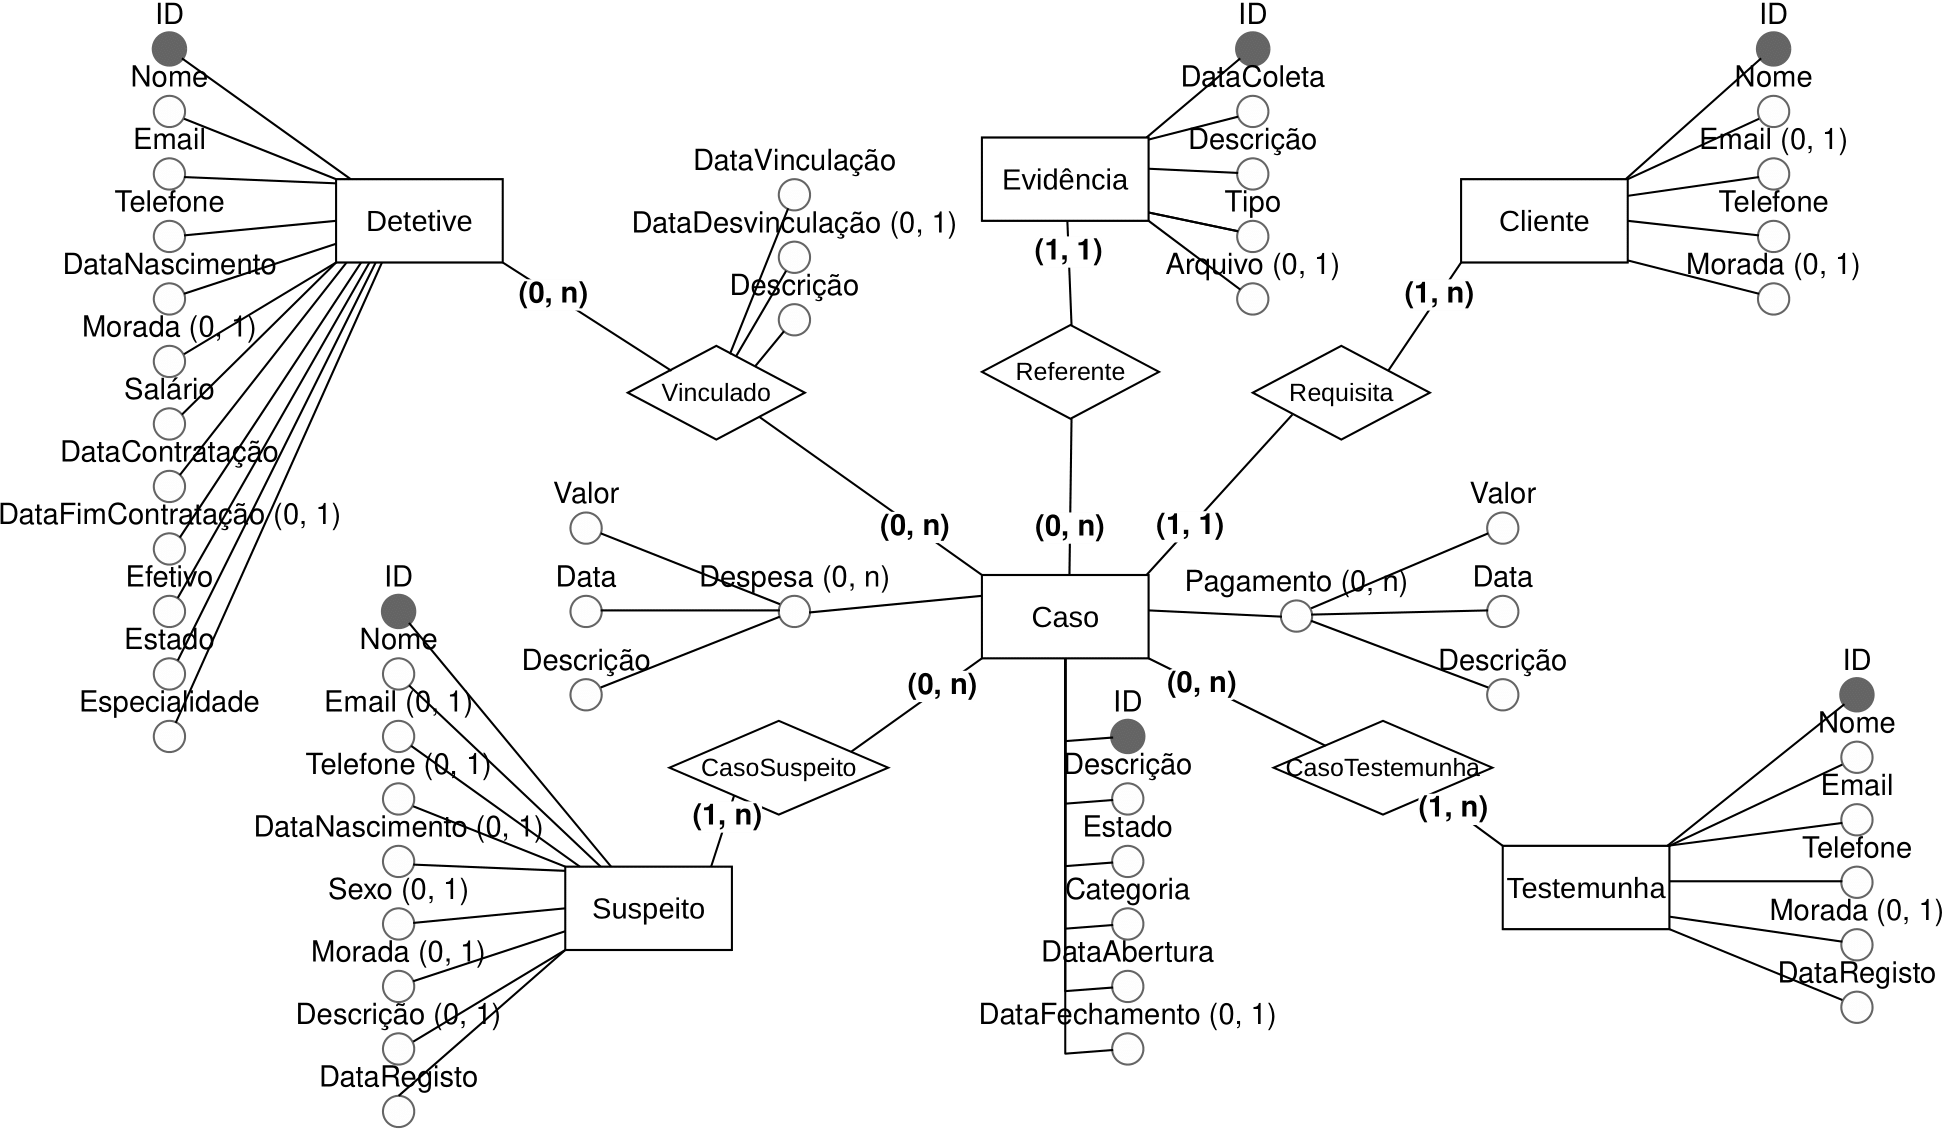
\includegraphics[scale=1.05, angle=270]{images/conceptual.png}
            \caption{Diagrama ER Conceptual}
            \label{fig:3.1}
        \end{figure}
        
        \loadgeometry{default}

%==========================================================================
% END MODELAÇÃO CONCEPTUAL
%==========================================================================

%==========================================================================
% BEGIN MODELAÇÃO LÓGICA
%==========================================================================

\chapter{Modelação Lógica}
    \label{sec:model_logica}

    \section{Construção e Validação do Modelo de Dados Lógico}

        Inicialmente, partimos do modelo conceptual, que representa os conceitos e relações do sistema de forma abstrata. Utilizámos o \textit{MySQL Workbench} para traduzir esses conceitos em estruturas de base de dados concretas, refletindo as entidades, atributos e relacionamentos identificados no modelo conceptual.

        Foram ajustados detalhes para otimizar a estrutura do banco de dados e garantir a sua eficiência e escalabilidade. Desde técnicas para garantir a normalização de dados, a definição de chaves primárias e estrangeiras, e a revisão de tipos de dados.
    
        No final do processo, o modelo lógico representa uma versão refinada e detalhada do sistema, pronta para ser implementada numa Base de Dados relacional. No entanto, é importante ressaltar que o modelo lógico não é uma representação final e imutável do sistema, mas sim uma etapa intermédia no processo de desenvolvimento de \textit{software}, sujeita a revisões e ajustes conforme novos requisitos são identificados.
        
    \clearpage
        
    \section{Apresentação e Explicação do Modelo Lógico Produzido}
        
        A construção do modelo lógico baseou-se intrinsecamente no modelo conceptual desenvolvido no capítulo anterior. Para tal, é necessário aplicar as regras de derivação do modelo de dados relacional.

        Primeiramente, cada entidade é convertida numa tabela e são definidos o tipo de dados dos atributos. Deste processo, obtemos as seguintes seis tabelas:

        \textbf{Caso}:
        \begin{itemize}
            \item Chave primária:
                \begin{itemize}
                    \item ID : INT
                \end{itemize}
            \item Chaves estrangeiras:
                \begin{itemize}
                    \item Cliente : INT
                    \item Categoria : INT
                    \item Estado : INT
                \end{itemize}
            \item Atributos:
                \begin{itemize}
                    \item Descrição : TEXT(2000)
                    \item DataAbertura : DATE
                    \item DataFechamento : DATE (Nulo)
                \end{itemize}
        \end{itemize}

        \clearpage

        \textbf{Detetive}:
        \begin{itemize}
            \item Chave primária:
                \begin{itemize}
                    \item ID : INT
                \end{itemize}
            \item Chaves estrangeiras:
                \begin{itemize}
                    \item Especialidade : INT
                    \item Estado : INT
                \end{itemize}
            \item Atributos:
                \begin{itemize}
                    \item Nome : VARCHAR(150)
                    \item Email : VARCHAR(320)
                    \item Telefone : VARCHAR(20)
                    \item DataNascimento : DATE
                    \item Morada : VARCHAR(250) (Nulo)
                    \item Salário : DECIMAL(10,2)
                    \item DataContratação : DATE
                    \item DataFimContratação : DATE (Nulo)
                    \item Efetivo : BIT
                \end{itemize}
        \end{itemize}

        \vspace{0.5cm}

        \textbf{Cliente}:
        \begin{itemize}
            \item Chave primária:
                \begin{itemize}
                    \item ID : INT
                \end{itemize}
            \item Chaves estrangeiras: Nenhuma
            \item Atributos:
                \begin{itemize}
                    \item Nome : VARCHAR(150)
                    \item Telefone : VARCHAR(20)
                    \item Email : VARCHAR(320) (Nulo)
                    \item Morada : VARCHAR(250) (Nulo)
                \end{itemize}
        \end{itemize}

        \clearpage

        \textbf{Suspeito}:
        \begin{itemize}
            \item Chave primária:
                \begin{itemize}
                    \item ID : INT
                \end{itemize}
            \item Chaves estrangeiras: Nenhuma
            \item Atributos:
                \begin{itemize}
                    \item Nome : VARCHAR(150)
                    \item Email : VARCHAR(320) (Nulo)
                    \item Telefone : VARCHAR(20) (Nulo)
                    \item DataNascimento : DATE (Nulo)
                    \item Sexo : CHAR(1) (Nulo)
                    \item Morada : VARCHAR(250) (Nulo)
                    \item Descrição : TEXT(1000) (Nulo)                    
                \end{itemize}
        \end{itemize}

        \vspace{0.5cm}

        \textbf{Testemunha}:
        \begin{itemize}
            \item Chave primária:
                \begin{itemize}
                    \item ID : INT
                \end{itemize}
            \item Chaves estrangeiras: Nenhuma
            \item Atributos:
                \begin{itemize}
                    \item Nome : VARCHAR(150)
                    \item Email : VARCHAR(320) (Nulo)
                    \item Telefone : VARCHAR(20) (Nulo)
                    \item Morada : VARCHAR(250) (Nulo)
                \end{itemize}
        \end{itemize}

        \clearpage
        \newgeometry{top=2cm}

        \textbf{Evidência}:
        \begin{itemize}
            \item Chave primária:
                \begin{itemize}
                    \item ID : INT
                \end{itemize}
            \item Chave estrangeira:
                \begin{itemize}
                    \item Caso : INT
                    \item Tipo : INT
                \end{itemize}
            \item Atributos:
                \begin{itemize}
                    \item DataColeta : DATE
                    \item Descrição : TEXT(1000)
                    \item Arquivo : VARCHAR(300) (Nulo)
                \end{itemize}
        \end{itemize}

        \vspace{0.2cm}

        A aplicação da regra de conversão de uma entidade conceptual em uma tabela deu origem ao seguinte modelo lógico (figura [\ref{fig:4.1}]):

        \vspace{0.1cm}

        \begin{figure}[!ht]
            \centering
            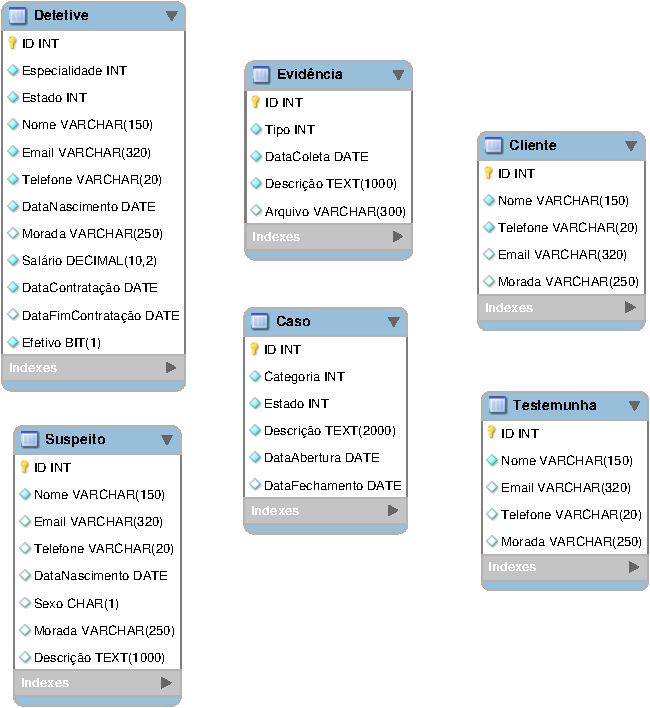
\includegraphics[scale=0.995]{images/modelo_logico/regra1.pdf}
            \caption{Diagrama ER Lógico após a aplicação da primeira regra de derivação}
            \label{fig:4.1}
        \end{figure}

        \loadgeometry{default}
        \clearpage
        
        Para a conversão de um \textbf{Relacionamento Binário de grau N:M}, a chave primária de cada entidade é utilizada para a composição da chave primária composta da tabela originada do relacionamento, e esta deve incluir os seus atributos, se existentes.

        Para os restantes relacionamentos é necessário a atribuição das chaves estrangeiras respetivas. Para tal, a chave primária da entidade do lado N é usada como chave estrangeira na entidade correspondente do lado 1.

        A regra de conversão do relacionamento de grau N:M originou as seguintes três tabelas:
        
        \textbf{Vinculação}:
        \begin{itemize}
            \item Chave primária composta:
                \begin{itemize}
                    \item Detetive : INT
                    \item Caso : INT
                    \item DataVinculação : DATETIME
                \end{itemize}
            \item Chaves estrangeiras:
                \begin{itemize}
                    \item Detetive : INT
                    \item Caso : INT
                \end{itemize}
            \item Atributos:
                \begin{itemize} 
                    \item DataDesvinculação : DATETIME (Nulo)
                    \item Descrição : TEXT(400)
                \end{itemize}
        \end{itemize}

        \vspace{0.5cm}

        \textbf{\textit{CasoSuspeito}}:
        \begin{itemize}
            \item Chave primária composta:
                \begin{itemize}
                    \item Caso : INT
                    \item Suspeito : INT
                \end{itemize}
            \item Chaves estrangeiras:
                \begin{itemize}
                    \item Caso : INT
                    \item Suspeito : INT
                \end{itemize}
            \item Atributos: Nenhum
        \end{itemize}

        \clearpage           
        
        \textbf{\textit{CasoTestemunha}}:
        \begin{itemize}
            \item Chave primária composta:
                \begin{itemize}
                    \item Caso : INT
                    \item Testemunha : INT
                \end{itemize}
            \item Chaves estrangeiras:
                \begin{itemize}
                    \item Caso : INT
                    \item Testemunha : INT
                \end{itemize}
            \item Atributos: Nenhum
        \end{itemize}

        \vspace{0.2cm}

        No fim desta conversão de relacionamentos binários de grau N:M e atribuição de chaves estrangeiras para os restantes relacionamentos, obtemos o modelo lógico apresentado na figura [\ref{fig:4.2}].

        \newgeometry{right=0.5cm,left=0.5cm,top=3cm,bottom=4cm}

        \begin{figure}
            \centering
            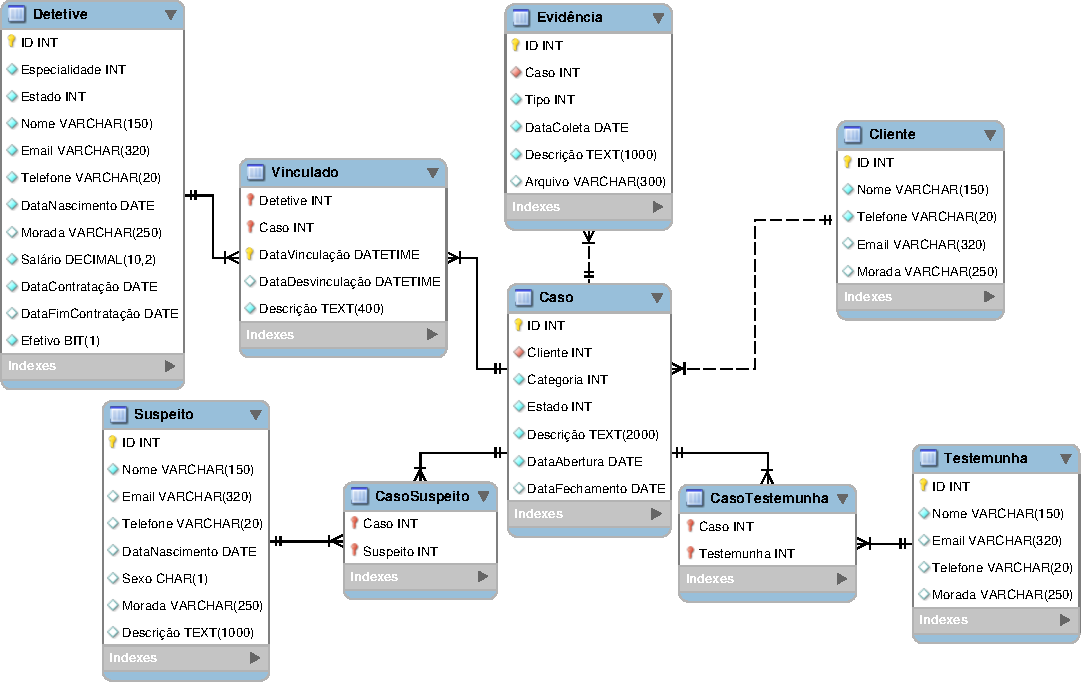
\includegraphics[scale=1,angle=0]{images/modelo_logico/regra2.pdf}
            \caption{Diagrama ER Lógico após a aplicação da segunda regra de derivação}
            \label{fig:4.2}
        \end{figure}

        \loadgeometry{default}

        No modelo conceptual, foram utilizados dois \textbf{atributos compostos multivalorados} na entidade “Caso”, de forma a registar pagamentos e despesas relativas ao mesmo. Estes atributos especiais resultam na formação de duas tabelas, cujas características são derivadas dos subatributos do atributo composto, e os mesmos formam a chave primária composta da respetiva tabela juntamente com a chave primária da tabela “Caso”. As quais:
        
        \textbf{Pagamento}:
        \begin{itemize}
            \item Chave primária composta:
                \begin{itemize}
                    \item Caso : INT
                    \item Descrição : TEXT(300)
                    \item Valor : DECIMAL(10,2)
                    \item Data : DATE
                \end{itemize}
            \item Chave estrangeira:
                \begin{itemize}
                    \item Caso : INT
                \end{itemize}
            \item Atributos: Nenhum
        \end{itemize}

        \vspace{0.5cm}

        \textbf{Despesa}:
        \begin{itemize}
            \item Chave primária composta:
                \begin{itemize}
                    \item Caso : INT
                    \item Descrição : TEXT(300)
                    \item Valor : DECIMAL(10,2)
                    \item Data : DATE
                \end{itemize}
            \item Chave estrangeira:
                \begin{itemize}
                    \item Caso : INT
                \end{itemize}
            \item Atributos: Nenhum
        \end{itemize}

        \vspace{0.5cm}

        Dada a conversão dos atributos multivalorados definidos no modelo conceptual, obtivemos o seguinte modelo lógico (figura [\ref{fig:4.3}]) com a adição de duas tabelas:
        \newgeometry{top=2cm,left=0cm,right=0cm,bottom=4cm}

        \clearpage
        \begin{figure}[!ht]
            \centering
            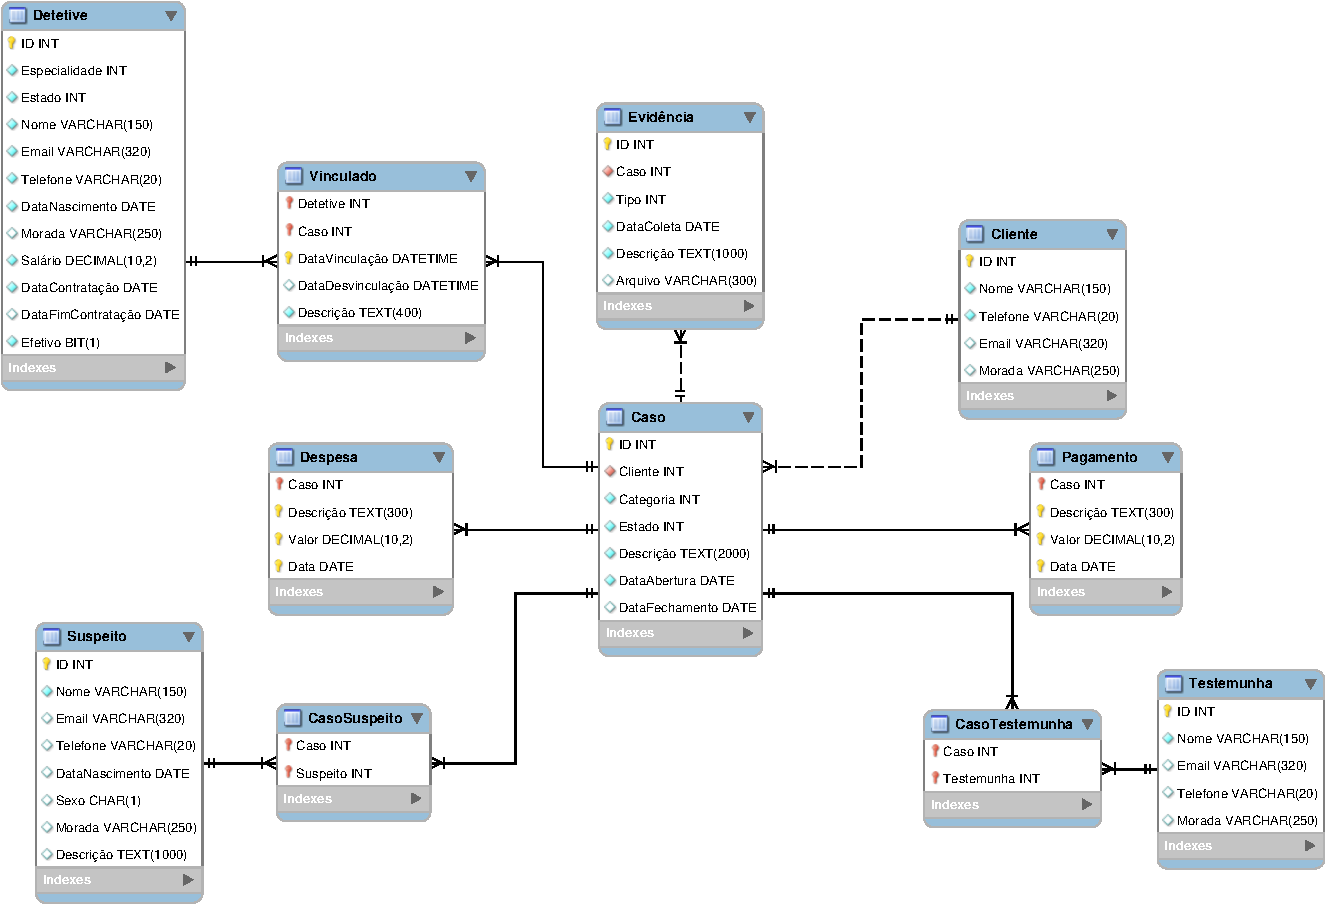
\includegraphics[scale=1, angle=270]{images/modelo_logico/regra3.pdf}
            \caption{Diagrama ER Lógico após a aplicação da terceira regra de derivação}
            \label{fig:4.3}
        \end{figure}
    
        \loadgeometry{default}

        \clearpage

        No processo de modelação lógica, foram adicionadas \textbf{entidades para o domínio de dados de atributos}, de forma a garantir uma uniformidade dos dados. Estas efetuam o mapeamento entre um identificador, representado por um número inteiro positivo, e uma designação, representado por um campo de texto. Para uma nomeação homogénea destas tabelas, utilizámos a seguinte nomenclatura: “\textit{EntidadeAtributo}”. Obtemos, assim, as seguintes cinco tabelas:

        \textbf{\textit{CasoCategoria}}:
        \begin{itemize}
            \item Chave primária:
                \begin{itemize}
                    \item ID : INT
                \end{itemize}
            \item Chave estrangeira: Nenhuma
            \item Atributos:
                \begin{itemize}
                    \item Designação : VARCHAR(75)
                \end{itemize}
        \end{itemize}

        \vspace{0.5cm}
        
        \textbf{\textit{CasoEstado}}:
        \begin{itemize}
            \item Chave primária:
                \begin{itemize}
                    \item ID : INT
                \end{itemize}
            \item Chave estrangeira: Nenhuma
            \item Atributos:
                \begin{itemize}
                    \item Designação : VARCHAR(20)
                \end{itemize}
        \end{itemize}

        \vspace{0.5cm}
        
        \textbf{\textit{DetetiveEspecialidade}}:
        \begin{itemize}
            \item Chave primária:
                \begin{itemize}
                    \item ID : INT
                \end{itemize}
            \item Chave estrangeira: Nenhuma
            \item Atributos:
                \begin{itemize}
                    \item Designação : VARCHAR(75)
                \end{itemize}
        \end{itemize}

        \clearpage
        
        \textbf{\textit{DetetiveEstado}}:
        \begin{itemize}
            \item Chave primária:
                \begin{itemize}
                    \item ID : INT
                \end{itemize}
            \item Chave estrangeira: Nenhuma
            \item Atributos:
                \begin{itemize}
                    \item Designação : VARCHAR(20)
                \end{itemize}
        \end{itemize}

        \vspace{0.5cm}
        
        \textbf{\textit{EvidênciaTipo}}:
        \begin{itemize}
            \item Chave primária:
                \begin{itemize}
                    \item ID : INT
                \end{itemize}
            \item Chave estrangeira: Nenhuma
            \item Atributos:
                \begin{itemize}
                    \item Designação : VARCHAR(20)
                \end{itemize}
        \end{itemize}

    \vspace{1cm}

    Após a aplicação das regras de derivação do modelo de dados relacional, obtemos o modelo lógico apresentado na figura [\ref{fig:4.4}].

    \textbf{Nota}: Consultar anexo \textit{\nameref{anexo:4}} para uma melhor visualização deste modelo.
    \newgeometry{top=0.1cm,left=0cm,right=0cm,bottom=0.1cm}

    \clearpage
    \begin{figure}[!ht]
        \centering
        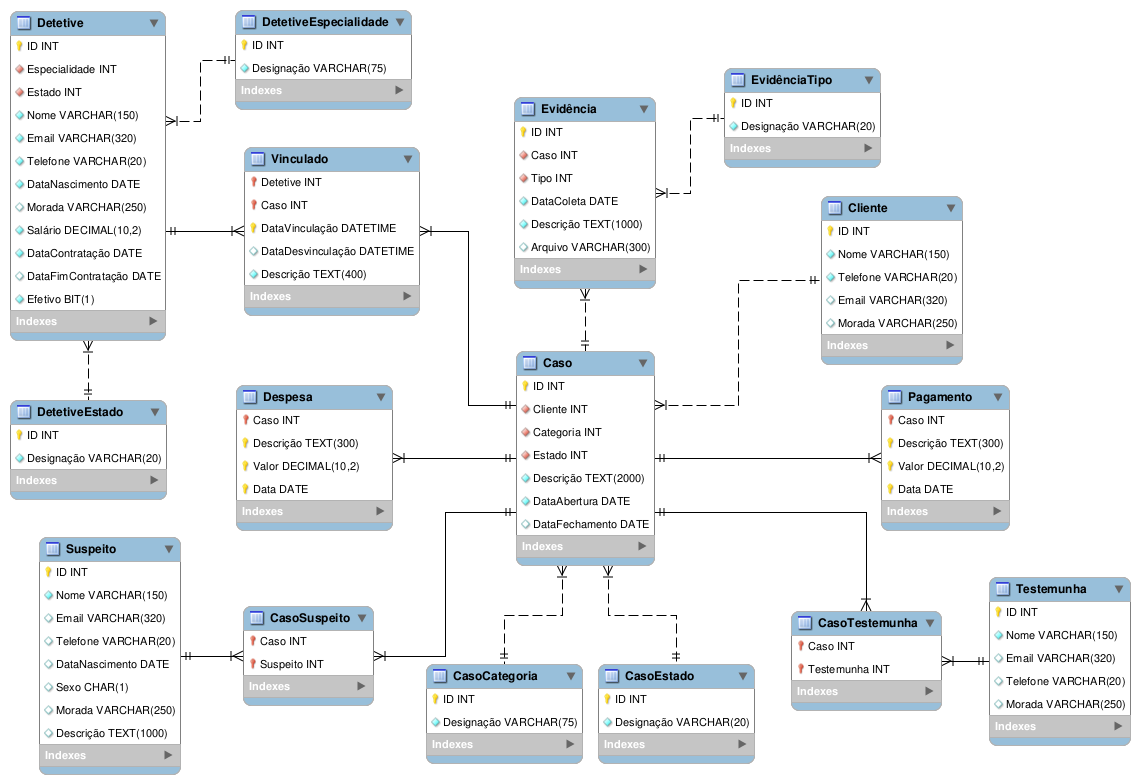
\includegraphics[scale=0.70, angle=270]{images/modelo_logico/final.png}
        \caption{Diagrama ER Lógico}
        \label{fig:4.4}
    \end{figure}

    \loadgeometry{default}

    \clearpage
    \newgeometry{top=2.5cm,bottom=3cm}
    \section{Normalização de Dados}
        De forma a garantir a normalização dos dados, é necessário considerar os seguintes pontos: \cite{DatabaseSystems} (Connolly \& Begg, 2015)
        \begin{itemize}
            \item Redução de Redundância
            \item Consistência dos Dados
            \item Facilidade de Manutenção
            \item Desempenho Aprimorado
        \end{itemize}
        O sistema de base de dados implementado visa a redução de redundância ao evitar a duplicação desnecessária de informações, proporcionando níveis de armazenamento mais económicos e evitando incongruências entre diferentes instâncias dos mesmos dados. Um exemplo da aplicação desta redução originou do relacionamento Caso e Suspeito, que, numa fase inicial de desenvolvimento, um suspeito estava associado a um único caso, no entanto, em um aprofundamento com os membros da CDC, concluiu-se que um suspeito tinha uma maior probabilidade de estar associado a vários casos. Após esta conclusão, o modelo foi amplificado para incluir uma relação derivada deste relacionamento, o que permite a associação de um suspeito a vários casos, evitando assim duplicações de suspeitos. O mesmo se aplicou com as entidades caso e testemunha, devido ao seu relacionamento similar ao exemplo anterior.

        Esta solução exemplificada promoveu a integridade dos dados e tornou mais fácil garantir que os dados estejam sempre corretos e atualizados, confirmando a consistência dos dados, que é fulcral à normalização destes.

        O sistema garante a facilidade de manutenção, gestão e escalonamento da plataforma, providenciando uma base ótima para estas ações, através de uma única responsabilidade para cada entidade e da organização estabelecida entre estas. Por exemplo, a criação de relações para o mapeamento de valores, tais como a categoria de um caso ou a área de especialização de um detetive, possibilita a facilidade de manutenção destes valores e endossa o escalonamento ao longo do crescimento da agência e do aperfeiçoamento na sua área de atuação.

        A plataforma demonstra padrões de centralização e padronização, permitindo aos seus utilizadores que tenham acesso às informações relevantes de forma rápida e precisa e, para além disso, a estrutura organizada do banco de dados facilita a implementação de medidas de controlo de acesso e segurança, através da definição de permissões de utilizadores específicas com base nas entidades e respetivos atributos, garantindo que apenas membros autorizados possam visualizar ou modificar determinadas informações.

        Em suma, o sistema demonstra um compromisso firme com a normalização de dados, garantindo eficiência, integridade e segurança. Ao evitar redundâncias, estabelecer relações claras entre entidades e implementar medidas de controlo de acesso, o sistema promove uma operação suave e escalável. Essa abordagem não apenas otimiza as operações atuais, mas também prepara a plataforma para um crescimento sustentável e contínuo.

    \loadgeometry{default}

    \clearpage
    \section{Validação do Modelo com Interrogações do Utilizador}
        \label{sec:val_model}
        
        Para assegurar a completa validade do modelo lógico de ER, foram selecionadas um conjunto de expressões algébricas derivadas dos requisitos relativos à manipulação de dados, de forma a permitirem a validação de uma grande totalidade das relações e relacionamentos estipulados no modelo. Estas serão aprofundadas nos parágrafos seguintes.

        \textbf{Nota}: Consultar anexos \textit{\nameref{anexo:5}} e \textit{\nameref{anexo:6}} para a visualização das entidades e expressões utilizadas na ferramenta ReLaX.

\clearpage

{\large\textbf{4.4.1 Aceder a identificadores de detetives que estão vinculados a um caso em específico (exemplo: ID do caso = 1), nessa instância.}}

\vspace{0.2cm}

A interrogação 1 baseou-se no requisito de manipulação número 12: \textit{“Dado o identificador do caso, deve ser possível aceder a todos os detetives que já estiveram envolvidos, bem como detetives envolvidos no momento.”}.

\vspace{0.2cm}

\begin{lstlisting}[escapechar=*]
*$\sigma$* (caso *$=$* 1 AND dataDesvinculacao *$=$* 'NULL') (vinculacao)
\end{lstlisting}

\begin{figure}[!ht]
    \centering
    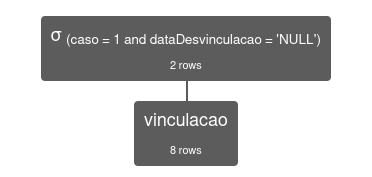
\includegraphics[scale=0.9]{images/relax/1.png}
    \caption{Representação gráfica da expressão em Álgebra Relacional 1.}
 \end{figure}
\vspace{0.2cm}

Esta expressão efetua uma seleção através do identificador único do caso e da data de desvinculação na entidade “vinculação”, desta forma é permitido aceder a detetives vinculados a um caso em específico nessa instância.

Ao substituir o sinal de igual pelo seu inverso em `\textit{dataDesvinculacao = 'NULL'}`, seria possível obter detetives que já estiveram vinculados ao caso, mas entretanto foram desvinculados deste.

Ao remover o termo da condição - `\textit{dataDesvinculacao = 'NULL'}` - originava uma expressão que retornava todos detetives que estão e estiveram associados a um caso em específico, ou seja todos os detetives envolvidos em um caso.

\clearpage %%\vspace{0.5cm}
{\large\textbf{4.1.2 Aceder a casos onde um detetive em específico (exemplo: ID do detetive = 1) está ativamente vinculado, nessa instância.}}

\vspace{0.2cm}

A interrogação 2 baseou-se no requisito de manipulação número 19: \textit{“Dado o identificador de um detetive, deve ser possível aceder a todos os casos em que esteve/está envolvido.”}.

\vspace{0.2cm}

\begin{lstlisting}[escapechar=*]
*$\sigma$* (detetive *$=$* 1 AND dataDesvinculacao *$=$* 'NULL') (vinculacao)
\end{lstlisting}

\begin{figure}[!ht]
    \centering
    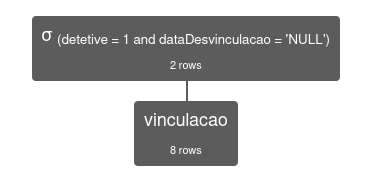
\includegraphics[scale=0.9]{images/relax/2.png}
    \caption{Representação gráfica da expressão em Álgebra Relacional 2.}
\end{figure}
\vspace{0.2cm}

Similarmente à expressão analisada anteriormente, é possível, através do identificador de um detetive, aceder aos casos onde este está/esteve vinculado. Neste cenário são apresentados casos onde o detetive se encontra ativamente vinculado a estes.

A obtenção de resultados conforme a atividade do detetive na investigação de um caso varia de acordo com as modificações do segundo termo da condição abordadas na primeira expressão algébrica estudada.

\clearpage %%\vspace{0.5cm}
{\large\textbf{4.1.3 Relatório completo de pagamentos com data, descrição e valor para um caso em específico (exemplo: ID do caso = 1).}}

\vspace{0.2cm}

A interrogação 3 baseou-se no requisito de manipulação número 49: \textit{“No encerramento de cada dia, o sistema deverá gerar um relatório que inclua todas as despesas e pagamentos efetuados. Este deve apresentar individualmente cada despesa e pagamento, se existirem, por caso. Adicionalmente, o relatório deve fornecer o somatório total de despesas, pagamentos, bem como os lucros ou prejuízos acumulados nesse dia.”}.

\vspace{0.2cm}

\begin{lstlisting}[escapechar=*]
*$\pi$* data, valor, descricao
*$\sigma$* (caso *$=$* 1) (pagamento)
\end{lstlisting}

\begin{figure}[!ht]
    \centering
    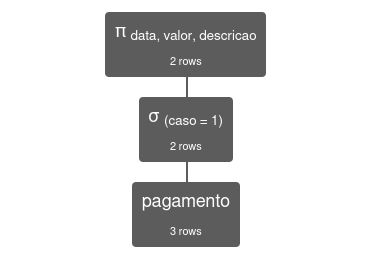
\includegraphics[scale=0.9]{images/relax/3.png}
    \caption{Representação gráfica da expressão em Álgebra Relacional 3.}
\end{figure}
\vspace{0.2cm}

A expressão algébrica número 3 permite a obtenção de todos os pagamentos efetuados relativos a um caso em específico, realizando uma projeção dos atributos data, valor e descrição, seguida de uma seleção da entidade “pagamento” através do identificador do caso.

Uma expressão algébrica para a obtenção de todas as despesas efetuadas relativas a um caso seria semelhante a expressão apresentada, com a diferença do acesso à entidade “despesa” em vez de “pagamento”, isto deve-se à conveniente similaridade dos atributos dessas entidades. 

\clearpage %%\vspace{0.5cm}
{\large\textbf{4.1.4 Estatísticas de casos abertos, fechados e arquivados numa semana específica (exemplo: de 14/03/2024 a 20/04/2024).}}

\vspace{0.2cm}

A interrogação 4 baseou-se no requisito de manipulação número 51: \textit{“No encerramento de cada semana, o sistema deverá gerar um relatório com informações e estatísticas relativas a novos casos abertos, fechados e/ou arquivados.”}.

\vspace{0.2cm}

\begin{lstlisting}[escapechar=*]
*$\pi$* caso.id, caso.dataAbertura, caso.dataFechamento, casoestado.designacao
((*$\sigma$* (dataAbertura *$\geq$* '14/03/2024' AND dataAbertura *$\leq$* '20/04/2024') OR
(dataFechamento *$\geq$* '14/03/2024' AND dataFechamento *$\leq$* '20/04/2024') (caso))
*$\bowtie$* caso.estado *$=$* casoestado.id (casoestado))
\end{lstlisting}

\begin{figure}[!ht]
    \centering
    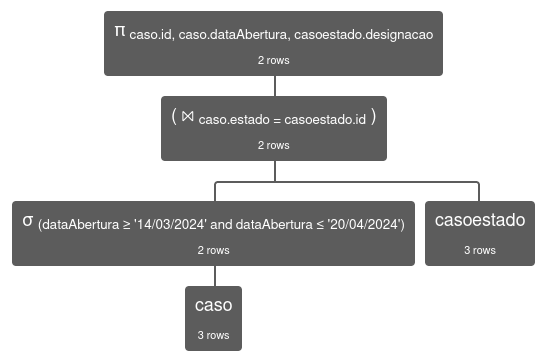
\includegraphics[scale=0.73]{images/relax/4.png}
    \caption{Representação gráfica da expressão em Álgebra Relacional 4.}
\end{figure}
\vspace{0.2cm}

A expressão algébrica número 4 obtém os identificadores de casos e o seu respetivo estado atual, onde estes são inicializados numa determinada semana. Esta serve para demonstrar o uso de entidades de mapeamento de valores, que, neste caso, foi utilizada a entidade “\textit{casoestado}” para mapear o atributo estado de um caso, representado por um número inteiro com a sua respetiva designação (“aberto”, “fechado” ou “arquivado”).

Uma otimização possível a esta expressão seria a truncação dos atributos \textit{id} e \textit{dataAbertura} da entidade “caso” antes da seleção através da data de abertura, desta forma, era aumentada a eficiência da expressão. A equipa de trabalho decidiu não incluir esta otimização de forma a manter a simplificação da expressão algébrica apresentada. 

\clearpage %%\vspace{0.5cm}
{\large\textbf{4.1.5 Apresentar os dados de um caso (exemplo: ID do caso = 1) - evidências, suspeitos e testemunhas - por ordem cronológica.}}

\vspace{0.2cm}

A interrogação 5 baseou-se no requisito de manipulação número 11: \textit{“Os dados relativos de cada caso - evidências, suspeitos e testemunhas - devem ser apresentados por ordem cronológica.”}.

\vspace{0.2cm}

\begin{lstlisting}[escapechar=*]
-- a) Obter todas as evidências relativas a um caso por ordem cronológica
*$\tau$* evidencia.dataColeta ASC
*$\sigma$* (caso *$=$* 1) (evidencia)

-- b) Obter todos os suspeitos relativos a um caso por ordem cronológica
*$\tau$* suspeito.dataRegisto ASC
*$\pi$* suspeito.nome, suspeito.telefone, suspeito.email, suspeito.dataNascimento, suspeito.sexo, suspeito.morada, suspeito.descricao, suspeito.dataRegisto
(*$\sigma$* (casosuspeito.caso *$=$* 1) (casosuspeito)
*$\bowtie$* casosuspeito.suspeito *$=$* suspeito.id (suspeito))

-- c) Obter todas as testemunhas relativas a um caso por ordem cronológica
*$\tau$* testemunha.dataRegisto ASC
*$\pi$* testemunha.nome, testemunha.telefone, testemunha.email, testemunha.morada, testemunha.dataRegisto
(*$\sigma$* (casotestemunha.caso *$=$* 1) (casotestemunha)
*$\bowtie$* casotestemunha.testemunha *$=$* testemunha.id (testemunha))
\end{lstlisting}

\begin{figure}[!ht]
    \centering
    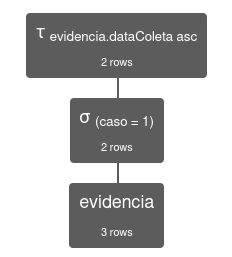
\includegraphics[scale=0.9]{images/relax/5-a.png}
    \caption{Representação gráfica da expressão em Álgebra Relacional 5.a)}
    \label{fig:4.5}
\end{figure}

\clearpage

\begin{figure}[!ht]
    \centering
    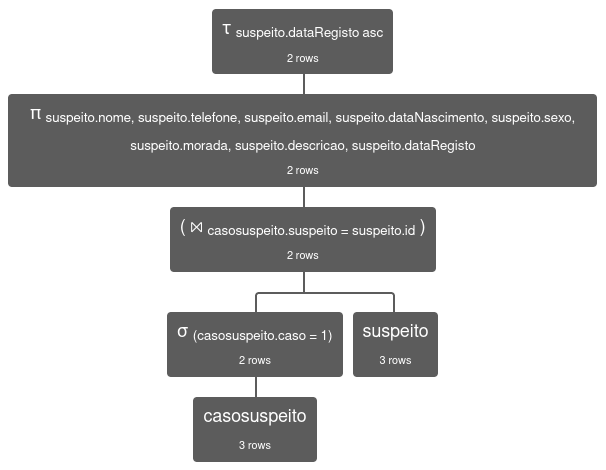
\includegraphics[scale=0.7]{images/relax/5-b.png}
    \caption{Representação gráfica da expressão em Álgebra Relacional 5.b)}
    \label{fig:4.6}
\end{figure}

\clearpage

\begin{figure}[!ht]
    \centering
    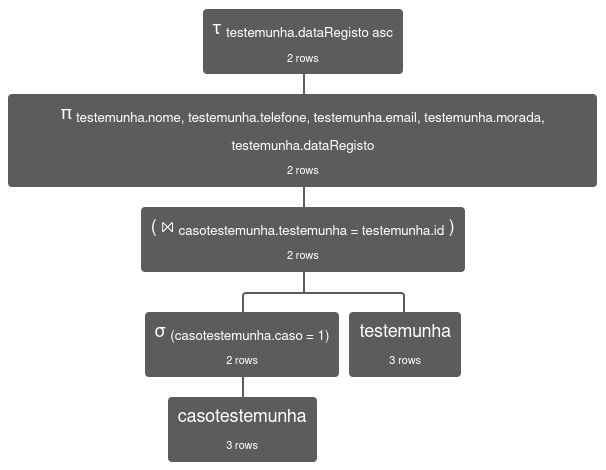
\includegraphics[scale=0.65]{images/relax/5-c.png}
    \caption{Representação gráfica da expressão em Álgebra Relacional 5.c)}
    \label{fig:4.7}
\end{figure}

Para apresentar os dados relativos a um caso em específico por ordem cronológica, as expressões foram divididas em três partes - a, b e c, respetivamente.

A primeira expressão (a) (figura [\ref{fig:4.5}]) é responsável por apresentar todos os registos de evidências relativo a um caso, através da seleção do identificador do caso. De seguida efetua-se a ordenação crescente pela data de coleta de evidência, de forma a garantir a ordem cronológica das evidências apresentadas.

Seguidamente, a expressão (b) (figura [\ref{fig:4.6}]) apresenta os dados das testemunhas de um determinado caso. Esta faz uma seleção através do identificador no caso na entidade “\textit{casotestemunha}”, obtendo assim todos os identificadores das testemunhas em questão. Após a truncação dos atributos relevantes às testemunhas, é feito a sua ordenação de forma crescente, através do atributo data de registo das testemunhas.

Por fim, a expressão (c) (figura [\ref{fig:4.7}]) apresenta os dados dos suspeitos de um determinado caso, similarmente à expressão (b) abordada no parágrafo anterior.

Seria possível a combinação das três expressões abordadas anteriormente de forma a obter uma única tabela como resultado. Para tal, era necessário unir as expressões anteriores e renomear os atributos \textit{testemunha.dataRegisto}, \textit{suspeito.dataRegisto} e \textit{evidencia.dataColeta} para um só para a reorganização dos registos através deste novo atributo unificado.

\clearpage %%\vspace{0.5cm}

{\large\textbf{4.1.6 Relatório diário de novas evidências, suspeitos e testemunhas de um caso em específico (exemplo: ID do caso = 1 e data = 20/03/2024).}}

\vspace{0.2cm}

A interrogação 6 baseou-se no requisito de manipulação número 50: \textit{“No encerramento de cada dia, o sistema deverá gerar um relatório para cada caso que inclua novas evidências, testemunhas e suspeitos.”}

\vspace{0.2cm}

\begin{lstlisting}[escapechar=*]
-- a) Obter as novas evidências relativas a um caso
*$\pi$* evidencia.id, evidencia.dataColeta, evidencia.descricao
*$\sigma$* (caso *$=$* 1 AND dataColeta *$=$* '20/03/2024') (evidencia)

-- b) Obter os novos suspeitos relativos a um caso
*$\pi$* suspeito.nome, suspeito.telefone, suspeito.email, suspeito.dataNascimento, suspeito.sexo, suspeito.morada, suspeito.descricao, suspeito.dataRegisto
*$\sigma$* (casosuspeito.caso *$=$* 1 AND suspeito.dataRegisto *$=$* '20/03/2024')
(casosuspeito *$\bowtie$* casosuspeito.suspeito *$=$* suspeito.id (suspeito))

-- c) Obter as novas testemunhas relativas a um caso
*$\pi$* testemunha.nome, testemunha.telefone, testemunha.email, testemunha.morada, testemunha.dataRegisto
*$\sigma$* (casotestemunha.caso *$=$* 1 AND testemunha.dataRegisto *$=$* '20/03/2024')
(casotestemunha *$\bowtie$* casotestemunha.testemunha *$=$* testemunha.id (testemunha))
\end{lstlisting}

\begin{figure}[!ht]
    \centering
    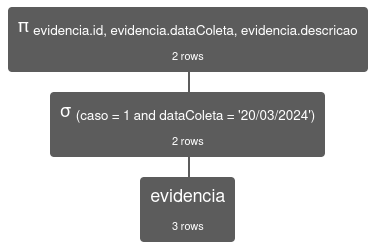
\includegraphics[scale=0.9]{images/relax/6-a.png}
    \caption{Representação gráfica da expressão em Álgebra Relacional 6.a)}
    \label{fig:4.8}
\end{figure}

\clearpage

Similarmente à interrogação anterior (5), esta foi dividida em três expressões algébricas (figuras [\ref{fig:4.8}], [\ref{fig:4.9}] e [\ref{fig:4.10}]), onde, em vez de uma ordenação cronológica, são apresentados dados através da seleção da data de coleta/registo relativa a cada entidade (evidências, suspeitos e testemunhas).

\begin{figure}[!ht]
    \centering
    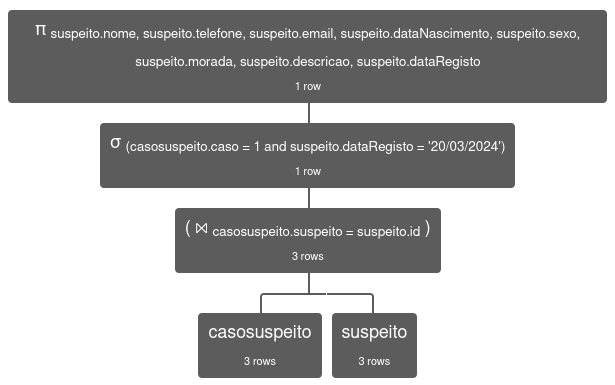
\includegraphics[scale=0.63]{images/relax/6-b.png}
    \caption{Representação gráfica da expressão em Álgebra Relacional 6.b)}
    \label{fig:4.9}
\end{figure}
\vspace{0cm}
\begin{figure}[!ht]
    \centering
    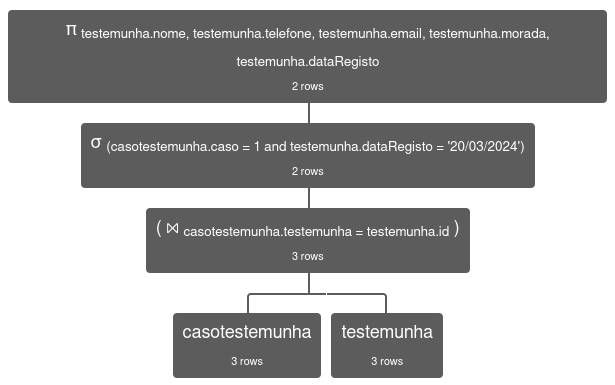
\includegraphics[scale=0.63]{images/relax/6-c.png}
    \caption{Representação gráfica da expressão em Álgebra Relacional 6.c)}
    \label{fig:4.10}
\end{figure}

\clearpage

De modo semelhante à unificação de expressões descrita anteriormente, estas três expressões da interrogação anterior podem ser unificadas de forma a apresentar uma única tabela como resultado, da seguinte maneira (figura [\ref{fig:4.11}]):

\vspace{0.2cm}
\begin{lstlisting}[escapechar=*]
*$\pi$* evidencia.caso, evidencia.id, evidencia.dataColeta, evidencia.descricao
*$\sigma$* (caso *$=$* 1 AND dataColeta *$=$* '20/03/2024') (evidencia)

*$\bowtie$* evidencia.caso *$=$* casosuspeito.caso

*$\pi$* casosuspeito.caso, suspeito.nome, suspeito.telefone, suspeito.email, suspeito.dataNascimento, suspeito.sexo, suspeito.morada, suspeito.descricao, suspeito.dataRegisto
*$\sigma$* (casosuspeito.caso *$=$* 1 AND suspeito.dataRegisto *$=$* '20/03/2024')
(casosuspeito *$\bowtie$* casosuspeito.suspeito *$=$* suspeito.id (suspeito))

*$\bowtie$* casosuspeito.caso *$=$* casotestemunha.caso

*$\pi$* casotestemunha.caso, testemunha.nome, testemunha.telefone, testemunha.email, testemunha.morada, testemunha.dataRegisto
*$\sigma$* (casotestemunha.caso *$=$* 1 AND testemunha.dataRegisto *$=$* '20/03/2024')
(casotestemunha *$\bowtie$* casotestemunha.testemunha *$=$* testemunha.id (testemunha))
\end{lstlisting}

\newgeometry{top=1cm,right=0cm,left=0cm,bottom=1cm}

\begin{figure}[!ht]
    \centering
    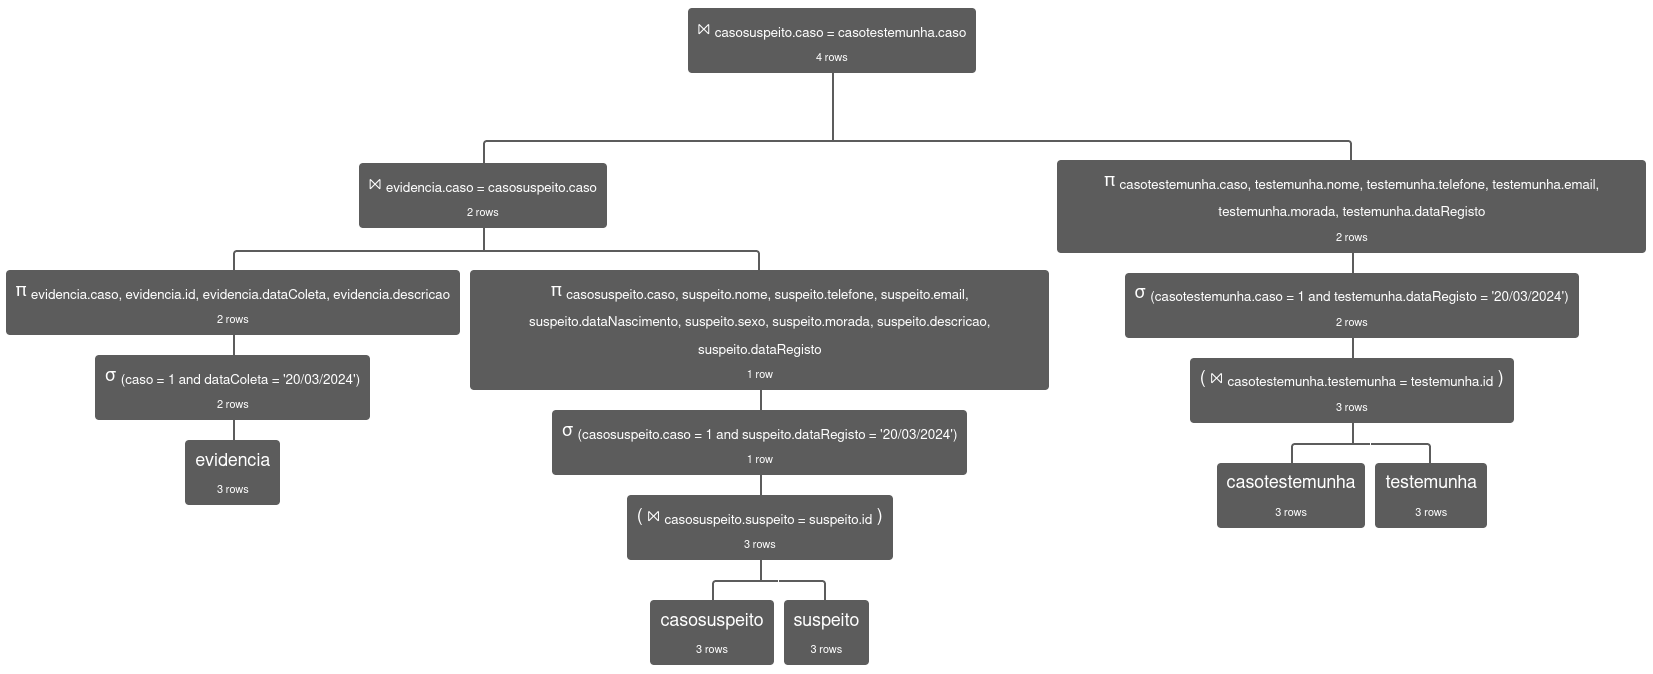
\includegraphics[scale=16, angle=270]{images/relax/6-example.png}
    \caption{Representação gráfica da expressão em Álgebra Relacional 6 (alternativa)}
    \label{fig:4.11}
\end{figure}

\loadgeometry{default}

%==========================================================================
% END MODELAÇÃO LÓGICA
%==========================================================================

%==========================================================================
% BEGIN IMPLEMENTAÇÃO FÍSICA
%==========================================================================

\chapter{Implementação Física}
\section{Apresentação e Explicação da Base de Dados Implementada}
\label{chap:impBD}
A implementação da Base de Dados efetuou-se através da tradução direta do modelo lógico previamente desenvolvido, com o acréscimo de restrições do domínio de valores e definição de valores predefinidos.

Primeiramente, foi definida a ordem na qual as tabelas devem ser criadas, de forma a garantir o cumprimento da regra de integridade referencial:

\begin{enumerate}
    \item Tabelas de mapeamento de valores: \textit{CasoEstado}, \textit{CasoCategoria}, \textit{DetetiveEspecialidade}, \textit{DetetiveEstado} e \textit{EvidênciaTipo};
    \item \textit{Cliente};
    \item \textit{Caso};
    \item \textit{Pagamento} e \textit{Despesa};
    \item \textit{Evidência}, \textit{Detetive}, \textit{Suspeito} e \textit{Testemunha};
    \item \textit Tabelas com múltiplos relacionamentos (1:N): \textit{Vinculado}, \textit{CasoSuspeito} e \textit{CasoTestemunha};
\end{enumerate}

Após a definição correta da ordem de criação das tabelas, demos início à construção do conjunto de instruções para a implementação da BD. A ordem definida acima não é estrita; para melhor legibilidade e organização, criámos imediatamente tabelas como \textit{CasoSuspeito} após a criação das tabelas \textit{Caso} e \textit{Suspeito}, já que os atributos referenciados pelas suas chaves estrangeiras já foram criados.

Para cada tabela, de acordo com as definições de metadados presentes na modelação lógica, designámos a sua chave primária e, se existirem, as respetivas chaves estrangeiras, o tipo de dados de cada atributo e a sua nulidade.

\clearpage

Para além disso, nesta fase, aproveitámos para criar restrições para a definição do domínio de valores de certos atributos, como, por exemplo, o atributo “sexo” da tabela \textit{Suspeito}, que garante que o valor deste atributo é 'M', 'F' ou nulo:

\vspace{0.4cm}
\begin{lstlisting}[escapechar=!]
CREATE TABLE IF NOT EXISTS Suspeito (
    -- (...)
    Sexo CHAR(1) NULL CHECK (Sexo IN ('M', 'F') OR Sexo IS NULL),
    -- (...)
);
\end{lstlisting}

De forma a agilizar a inserção de registos em certas tabelas, definimos valores predefinidos para certos atributos, como, por exemplo, o atributo “DataVinculação” da tabela \textit{Vinculado}, que permite a atribuição automática da data atual em uma vinculação de um detetive a um caso:

\vspace{0.4cm}
\begin{lstlisting}[escapechar=!]
CREATE TABLE IF NOT EXISTS Vinculado (
    -- (...)
    DataVinculação DATETIME NOT NULL DEFAULT CURRENT_TIMESTAMP,
    -- (...)
);
\end{lstlisting}

Também, para agilizar a inserção de registos, definimos um incremento sequencial automático das chaves primárias em tabelas onde consideramos pertinente implementar esta funcionalidade, como, por exemplo, na chave primária da tabela \textit{Caso}:   

\vspace{0.4cm}
\begin{lstlisting}[escapechar=!]
CREATE TABLE IF NOT EXISTS Caso (
    ID INT NOT NULL AUTO_INCREMENT,
    -- (...)
    PRIMARY KEY (ID),
    -- (...)
);
\end{lstlisting}

Após este processo, considerámos o \textit{script} de implementação da Base de Dados como completo. Para consultar este esquema físico produzido, confira o anexo \textit{\nameref{anexo:8}}.

\clearpage
\section{Criação de Utilizadores da Base de Dados}

    Para além do administrador da base de dados, Agatha Christie, o sistema deve garantir dois tipos de utilizador, com as respetivas permissões:
    \begin{itemize}
        \item \textbf{Detetive efetivo} - Visualiza, cria e modifica registos. Baseado nos requisitos de controlo \textbf{40} \textit{“O sistema deve garantir que apenas os detetives que estão vinculados a um determinado caso, podem alterar os dados relativos ao mesmo.”} e \textbf{42} \textit{“O sistema deve oferecer acesso aos dados de um caso aberto apenas aos detetives a si associados e a Agatha Christie.”};
        \item \textbf{Detetive estagiário} - Visualiza registos. Baseado no requisito de controlo \textbf{41} \textit{“O sistema deve garantir que os detetives estagiários apenas podem ler dados relativos a casos não abertos, ou seja, casos fechados e arquivados.”}.
    \end{itemize}

    Do seguinte modo, foram criados os seguintes utilizadores, detetive efetivo e estagiário, respetivamente:

    \vspace{0.4cm}
    \begin{lstlisting}[escapechar=!]
GRANT SELECT, INSERT, UPDATE ON cdc.* TO 'detetive1'!@!'localhost';

GRANT SELECT ON cdc.* TO 'estagiario5'!@!'localhost';
    \end{lstlisting}

    De forma a garantir o cumprimento total das restrições de permissões mencionadas nos requisitos 40, 41 e 42, ter-se-ia de recorrer ao uso de \textit{software} adicional, que, através do estado do detetive e/ou do estado do caso, determina, com o uso de instruções SQL, se a dada operação que o utilizador quer efetuar é, de facto, permitida, e, se tal for, permitir a sua execução no SBD.

    A estrutura de permissões implementada para os diferentes tipos de detetives da consultoria visa a segurança e a confidencialidade dos dados.

    Para a visualização do \textit{script} utilizado na criação dos utilizadores e definição das respetivas permissões, consulte o anexo \textit{\nameref{anexo:9}}.

\clearpage
\newgeometry{top=3cm}

\section{Povoamento da Base de Dados}

O povoamento da Base de Dados deu-se através da conversão manual dos registos físicos da CDC para um \textit{script} com instruções pertencentes ao conjunto DML, mais especificamente, instruções \textit{INSERT INTO}.

Assim como no subcapítulo \textit{\nameref{chap:impBD}}, a ordem na qual os registos são inseridos é fundamental para o povoamento correto da BD, assim como o cumprimento das restrições implementadas, desde o uso correto de chaves estrangeiras e o respeito dos domínios de valores estabelecidos.

Na inserção de clientes, exemplificamos o uso do incremento sequencial automático previamente desenvolvido, omitindo, assim, o identificador do cliente no seu registo.

Para além deste \textit{script} SQL, foi ainda implementado um programa em \textit{Python}, que exemplifica a execução de instruções SQL no servidor da BD. Este começa por, através do \textit{package mysql.connector}, estabelecer uma conexão com o servidor, e inicializa um objeto cursor para execução de \textit{queries}. De seguida, são introduzidos cinco clientes na BD, similarmente como no povoamento descrito anteriormente. Estes clientes são apresentados no terminal através de uma \textit{query} que efetua a seleção dos últimos cinco clientes criados através da ordenação decrescente do seus identificadores. Por fim, o cursor e a conexão são encerrados, respetivamente.

Para consultar o \textit{script} SQL e o programa \textit{Python}, por favor confira os respetivos anexos \textit{\nameref{anexo:10}} e \textit{\nameref{anexo:11}}.

\section{Cálculo do Espaço da Base de Dados}

Para o cálculo do espaço de armazenamento da BD, calculámos a dimensão inicial com um registo por tabela.

Para a obtenção dos tamanhos de cada tipo de dados, recorremos à secção \textit{13.7 Data Type Storage Requirements} do Manual de Referência \textit{MySQL 8.0} \cite{MySQLManual}. Neste cálculo, estipulámos que os caracteres utilizados em campos de texto têm correspondência direta na tabela ASCII, ou seja, estes ocupam um \textit{byte} por caractere.

Deste modo, obtemos uma dimensão inicial total de 8773 \textit{bytes}. Ao longo dos anos, a CDC observou uma taxa de crescimento anual média de 20\%, este crescimento resultaria num acréscimo de, aproximadamente, 1755 \textit{bytes} ($8773 \times 0.20$) do espaço de armazenamento da Base de Dados, por ano.

Para consultar a folha de cálculo utilizada, confira o anexo \textit{\nameref{anexo:12}}.

\loadgeometry{default}

\begin{figure}[!ht]
    \centering
    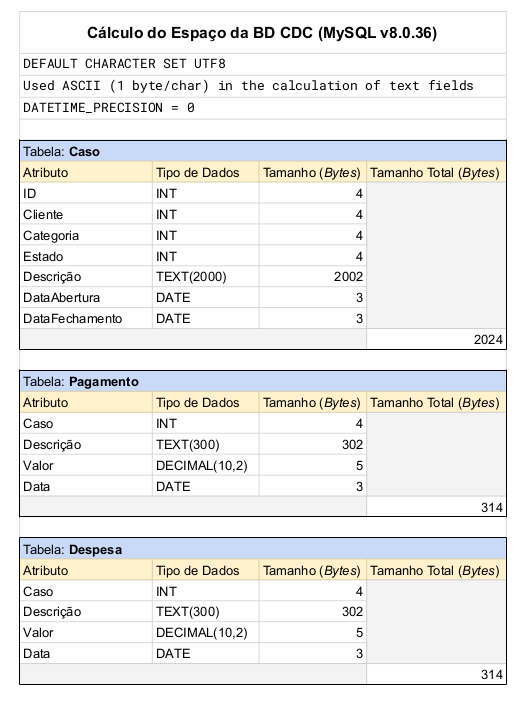
\includegraphics[scale=0.83]{images/armazenamento/1.png}
    \caption{Cálculo do Espaço de Armazenamento da BD}
    \label{fig:5.1}
\end{figure}

\begin{figure}[!ht]
    \centering
    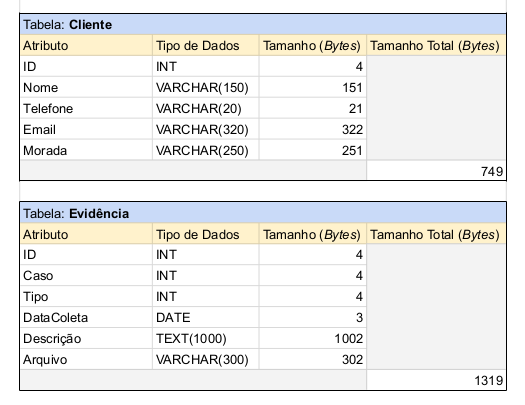
\includegraphics[scale=0.83]{images/armazenamento/2.png}
    \caption{Cálculo do Espaço de Armazenamento da BD}
    \label{fig:5.2}
\end{figure}

\begin{figure}[!ht]
    \centering
    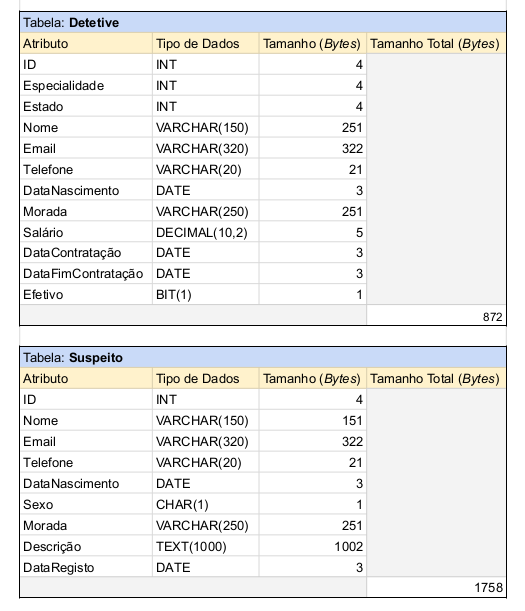
\includegraphics[scale=0.83]{images/armazenamento/3.png}
    \caption{Cálculo do Espaço de Armazenamento da BD}
    \label{fig:5.3}
\end{figure}

\begin{figure}[!ht]
    \centering
    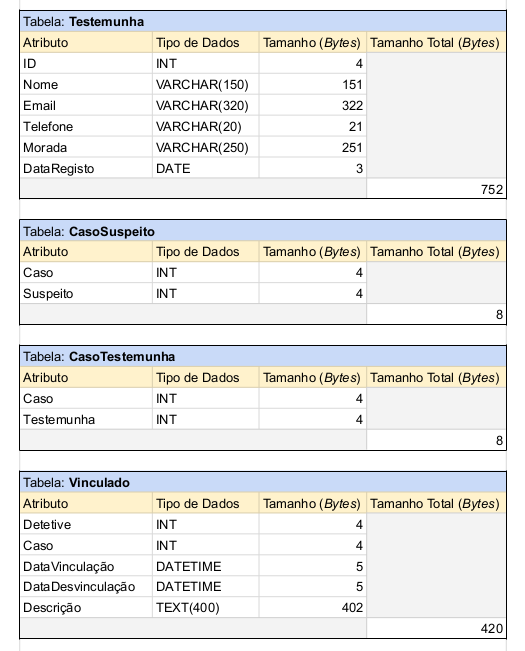
\includegraphics[scale=0.83]{images/armazenamento/4.png}
    \caption{Cálculo do Espaço de Armazenamento da BD}
    \label{fig:5.4}
\end{figure}

\begin{figure}[!ht]
    \centering
    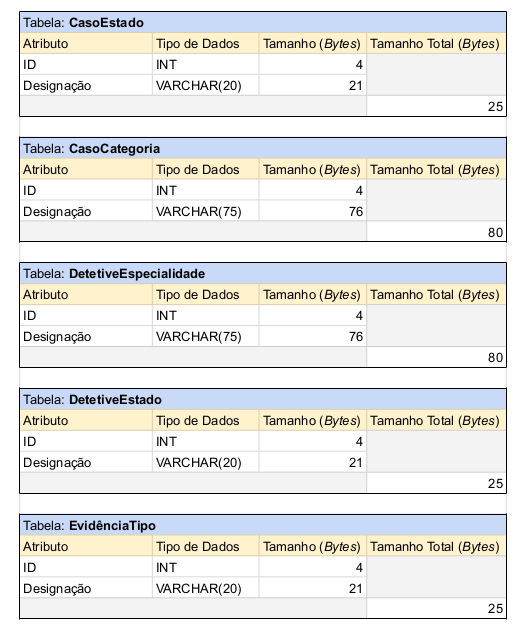
\includegraphics[scale=0.83]{images/armazenamento/5.png}
    \caption{Cálculo do Espaço de Armazenamento da BD}
    \label{fig:5.5}
\end{figure}

\clearpage

\section{Definição e Caracterização de Vistas de Utilização em SQL}

Com o objetivo de facilitar e otimizar as consultas dos dados aos utilizadores, foram implementadas as seguintes vistas de utilização:

\textit{\textbf{TodosSuspeitos}}

A vista \textit{TodosSuspeitos} apresenta todos os suspeitos registados na agência, através da seleção de todos os atributos dos registos da tabela \textit{Suspeito}.

\vspace{0.4cm}
\begin{lstlisting}
DELIMITER //
CREATE VIEW TodosSuspeitos AS
    SELECT * FROM Suspeito;
//
DELIMITER ;
\end{lstlisting}

\textit{\textbf{CasosAtivos}}

A vista \textit{CasosAtivos} apresenta todos os casos ativos da agência, em um determinado momento, através da filtragem onde o estado do caso se encontra em aberto. Nesta, é feita a junção dos atributos \textit{Estado} e \textit{Categoria} com as respetivas tabelas de mapeamento de valores, de forma a melhorar a apresentação da tabela resultado desta vista.

\vspace{0.4cm}
\begin{lstlisting}
DELIMITER //
CREATE VIEW CasosAtivos AS
    SELECT
        C.ID AS CasoID,
        C.Descrição,
        C.DataAbertura,
        CC.Designação AS Categoria,
        CL.Nome AS 'Nome do cliente',
        CL.Telefone AS 'Telefone do cliente',
        CL.Email AS 'Email do cliente'
    FROM Caso AS C
    INNER JOIN Cliente AS CL
    ON C.Cliente = CL.ID
    INNER JOIN CasoCategoria AS CC
    ON C.Categoria = CC.ID
    WHERE
        C.Estado = 1; -- 'aberto'
//
DELIMITER ;
\end{lstlisting}

\clearpage

\textit{\textbf{DetetivesAtivos}}

Similarmente a vista apresentada anteriormente, a vista \textit{DetetivesAtivos} apresenta todos os casos ativos da agência, em um determinado momento,
através da filtragem onde o estado do detetive se encontra como contratado. Nesta, é feita a junção do atributo \textit{Especialidade} com a respetiva tabela de mapeamento de valores, \textit{DetetiveEspecialidade}, de forma a melhorar a apresentação da tabela resultado desta vista.

\vspace{0.4cm}
\begin{lstlisting}
DELIMITER //
CREATE VIEW DetetivesAtivos AS
    SELECT
        D.ID AS DetetiveID,
        D.Nome,
        D.Email,
        D.Telefone,
        D.DataNascimento,
        D.Morada,
        D.Salário,
        D.DataContratação,
        D.Efetivo,
        DE.Designação AS Especialidade
    FROM Detetive AS D
    JOIN DetetiveEspecialidade AS DE
    ON D.Especialidade = DE.ID
    WHERE
        D.Estado = 1; -- 'contratado'
//
DELIMITER ;
\end{lstlisting}

\clearpage

\section{Tradução das Interrogações do Utilizador para SQL}

\textbf{Nota}: Para consultar as \textit{queries} desenvolvidas, confira o anexo \textit{\nameref{anexo:13}}.

{\large\textbf{5.6.1 Aceder a identificadores de detetives que estão vinculados a um caso em específico (exemplo: ID do caso = 1), nessa instância.}}

A primeira \textit{query} SQL foi obtida através da tradução direta da expressão AR previamente apresentada no subcapítulo \textit{\nameref{sec:val_model}}. Esta efetua a seleção de todos atributos da tabela \textit{Vinculado} onde o identificador do caso é igual a um e a data de desvinculação é nula, obtendo, assim, os identificadores dos detetives ativamente vinculados, bem como a descrição e data de vinculação.

\vspace{0.4cm}
\begin{lstlisting}[escapechar=!]
SELECT * FROM Vinculado
	WHERE Caso = 1 AND DataDesvinculação IS NULL;
\end{lstlisting}

{\large\textbf{5.6.2 Aceder a casos onde um detetive em específico (exemplo: ID do detetive = 1) está ativamente vinculado, nessa instância.}}

Similarmente à \textit{query} anterior, a segunda \textit{query} foi obtida através da tradução direta da correspondente expressão AR, e esta apresenta todos os casos onde um detetive está ativamente vinculado através do filtragem do seu identificador e da data de desvinculação.

\vspace{0.4cm}
\begin{lstlisting}[escapechar=!]
SELECT * FROM Vinculado
	WHERE Detetive = 1 AND DataDesvinculação IS NULL;
\end{lstlisting}

{\large\textbf{5.6.3 Relatório completo de pagamentos com data, descrição e valor para um caso em específico (exemplo: ID do caso = 1).}}

A tradução da expressão AR permitiu a obtenção da terceira \textit{query}, a qual apresenta a data, valor e descrição de todos os pagamentos referentes a um caso em específico.

\vspace{0.4cm}
\begin{lstlisting}[escapechar=!]
SELECT Data, Valor, Descrição FROM Pagamento
	WHERE Caso = 1;
\end{lstlisting}

\clearpage

{\large\textbf{5.6.4 Estatísticas de casos abertos, fechados e arquivados numa semana específica (exemplo: de 14/03/2024 a 20/04/2024).}}

A tradução direta da expressão AR facilmente permitiu a obtenção da \textit{query} nº 4, nesta é efetuado a operação SQL \textit{INNER JOIN} para obter a designação do estado do caso e, a partir da operação \textit{WHERE}, são apresentados apenas os casos cuja data de abertura ou de fecho se encontram entre o intervalado das datas dadas como exemplo. Em alternativa, poderia-se usar a função SQL \textit{WEEK}, que retorna o número da semana da data passada como argumento, deste modo, o utilizador apenas precisava de especificar o número da semana em vez do intervalo de datas.

\vspace{0.4cm}
\begin{lstlisting}[escapechar=!]
SELECT C.ID, C.DataAbertura, C.DataFechamento, CE.Designação
	FROM Caso AS C
    INNER JOIN CasoEstado AS CE
    ON C.Estado = CE.ID
	WHERE (C.DataAbertura >= '2024-03-14' AND C.DataAbertura <= '2024-04-20')
		OR (C.DataFechamento >= '2024-03-14' AND C.DataFechamento <= '2024-04-20');
\end{lstlisting}

{\large\textbf{5.6.5 Apresentar os dados de um caso (exemplo: ID do caso = 1) - evidências, suspeitos e testemunhas - por ordem cronológica.}}

Assim como nas expressões AR previamente apresentadas, esta interrogação foi também divida em três \textit{queries} SQL, que originam três tabelas resultado - evidências, suspeitos e testemunhas -, relativas a um caso, e por ordem cronológica.

\vspace{0.4cm}
\begin{lstlisting}[escapechar=!]
SELECT * FROM Evidência
	WHERE Caso = 1
	ORDER BY DataColeta ASC;

SELECT S.* FROM Suspeito AS S
	INNER JOIN CasoSuspeito AS CS
    ON CS.Caso = 1
    ORDER BY S.DataRegisto ASC;

SELECT T.* FROM Testemunha AS T
	INNER JOIN CasoTestemunha AS CT
    ON CT.Caso = 1
    ORDER BY T.DataRegisto ASC;
\end{lstlisting}

\clearpage

{\large\textbf{5.6.6 Relatório diário de novas evidências, suspeitos e testemunhas de um caso em específico (exemplo: ID do caso = 1 e data = 20/03/2024).}}

Assim como no subcapítulo \textit{\nameref{sec:val_model}}, serão apresentadas duas versões da implementação em SQL da interrogação nº 6.

Na primeira versão, através da tradução direta das expressões AR, foram obtidas três \textit{queries} SQL que apresentam como tabelas de resultado, as vinculações, suspeitos e testemunhas relativas a um caso em específico numa determinada data. Para a apresentação do relatório diário, em vez de se filtrar a data especifica ('2024-03-20', no exemplo apresentado), poderia-se usufruir do uso da função SQL \textit{CURRENT\_DATE}.

\vspace{0.4cm}
\begin{lstlisting}[escapechar=!]
SELECT ID, DataColeta, Descrição FROM Evidência
	WHERE Caso = 1
		AND DataColeta = '2024-03-20';

SELECT S.* FROM Suspeito AS S
	INNER JOIN CasoSuspeito AS CS
    ON CS.Caso = 1
    WHERE S.DataRegisto = '2024-03-20';

SELECT T.* FROM Testemunha AS T
	INNER JOIN CasoTestemunha AS CT
    ON CT.Caso = 1
    WHERE T.DataRegisto = '2024-03-20';
\end{lstlisting}

\vspace{1cm}

A versão alternativa a interrogação nº 6, exemplifica como as três \textit{queries} SQL anteriores poderiam ser combinadas em uma só. Esta \textit{query} foi obtida através da tradução da expressão AR previamente apresentada, com exceção da criação uma tabela auxiliar \textit{Target} que guarda os atributos \textit{Data} e \textit{Caso} para as filtragens e junções seguintes, e do uso da operação \textit{LEFT JOIN} em vez da junção natural, ao combinar os resultados das três tabelas resultado em uma só. Esta \textit{query} tem um comportamento similar a expressão AR apresentada com exceção
na apresentação da tabela resultado final.

\clearpage
\newgeometry{top=0.8cm}

\vspace{0.4cm}
\begin{lstlisting}[escapechar=!]
WITH Target AS (
    SELECT
        '2024-03-20' AS Data,
        '1' AS Caso
),
ES AS (
    SELECT
        E.Caso AS E_Caso,
        E.ID AS E_ID,
        E.Tipo AS E_Tipo,
        E.Descrição AS E_Descrição,
        E.Arquivo AS E_Arquivo
    FROM Evidência AS E, Target
        WHERE E.Caso = Target.Caso
            AND E.DataColeta = Target.Data
),
SS AS (
    SELECT
        CS.Caso AS S_Caso,
        S.ID AS S_ID,
        S.Nome AS S_Nome,
        S.Email AS S_Email,
        S.Telefone AS S_Telefone,
        S.DataNascimento AS S_DataNascimento,
        S.Sexo AS S_Sexo,
        S.Morada AS S_Morada,
        S.Descrição AS S_Descrição
    FROM Suspeito AS S, Target
        INNER JOIN CasoSuspeito AS CS
        ON CS.Caso = Target.Caso
        WHERE S.DataRegisto = Target.Data
),
TS AS (
    SELECT
        CT.Caso AS T_Caso,
        T.Nome AS T_Nome,
        T.Email AS T_Email,
        T.Telefone AS T_Telefone,
        T.Morada AS T_Morada
    FROM Testemunha AS T, Target
        INNER JOIN CasoTestemunha AS CT
        ON CT.Caso = Target.Caso
        WHERE T.DataRegisto = Target.Data
),
Result AS (
	SELECT * FROM ES
        LEFT JOIN SS
        ON ES.E_Caso = SS.S_Caso
        LEFT JOIN TS
        ON ES.E_Caso = TS.T_Caso
)
-- SELECT * FROM Result;
\end{lstlisting}

\loadgeometry{default}

\section{Indexação do Sistema de Dados}

A indexação permite otimizar as operações de consulta dos dados. Um dos aspetos destacados na análise de viabilidade foi a redução do tempo que os detetives necessitam para buscar informações sobre evidências e outros detetives. Estas indexações visam diretamente atender a essa necessidade, melhorando a eficácia das investigações. Após uma análise, criámos três indexações com os seguintes propósitos:

Implementámos uma indexação na coluna \textit{Caso}, que é uma chave estrangeira na tabela \textit{Evidência}, com o objetivo de facilitar a pesquisa de evidências. Esta melhoria é crucial para a resolução dos casos, uma vez que permite uma maior eficiência na obtenção de informações importantes. 

\vspace{0.4cm}
\begin{lstlisting}[escapechar=!, numbers=none]
CREATE INDEX idx_Caso ON Evidência (Caso);
\end{lstlisting}
\vspace{0.6cm}

Criámos a indexação \textit{idx\_telefone} na tabela \textit{Detetive}, especificamente na coluna \textit{Telefone}, para otimizar as consultas relacionadas aos números de telefone dos detetives. Esta decisão foi tomada porque, no âmbito das operações diárias, é fundamental ter uma maneira rápida e eficiente de contactar os detetives.

\vspace{0.4cm}
\begin{lstlisting}[escapechar=!, numbers=none]
CREATE INDEX idx_telefone ON Detetive (Telefone);
\end{lstlisting}
\vspace{0.6cm}

Para justificar a criação do índice \textit{idx\_dataDesvinculação} na tabela \textit{Vinculado} com base na coluna \textit{dataDesvinculação}, podemos mencionar a necessidade de melhorar o desempenho das consultas que frequentemente filtram ou ordenam os resultados por esta coluna. Além disso, ao utilizarmos várias \textit{views} e \textit{stored procedures} que dependem de consultas rápidas e eficientes sobre a data de desvinculação, a criação deste índice torna-se essencial.

\vspace{0.4cm}
\begin{lstlisting}[escapechar=!, numbers=none]
CREATE INDEX idx_dataDesvinculação ON Vinculado (DataDesvinculação);
\end{lstlisting}
\vspace{0.6cm}

\textbf{Nota}: Para consultar o \textit{script} para a indexação da BD confira o anexo \textit{\nameref{anexo:14}}.

\clearpage

\newgeometry{top=3cm}

\section{Implementação de procedimentos, funções e gatilhos}

A implementação de procedimentos, funções e gatilhos em BD é essencial para melhorar a eficiência, a integridade e a automatização.
Procedimentos e funções permitem a reutilização de código, facilitando operações complexas e repetitivas de forma padronizada. Gatilhos permitem executar ações automaticamente, o que garante uma melhor consistência e integridade dos dados.

\subsection{Procedimentos}

Para a execução de certos requisitos de manipulação, recorremos ao uso de procedimentos, de forma a agilizar a execução destes.

\textbf{Nota}: Para consultar os procedimentos implementados, confira os anexos \textit{\nameref{anexo:15}} e \textit{\nameref{anexo:16}}.

Deste modo, alguns dos procedimentos criados são:

\textit{\textbf{ConsultarDetetivesCaso}}

Este procedimento foi criado de forma a melhorar a eficiência e automatização da BD para a obtenção, através do identificador de um caso, de todos os detetives que já estiveram envolvidos, bem como os que se encontram ativamente vinculados neste caso. Este procedimento baseia-se no requisito nº \textbf{12} -
\textit{“Dado o identificador
do caso, deve ser possível aceder a todos os detetives que já estiveram envolvidos, bem como
detetives envolvidos no momento.”} - e uma derivação deste já foi estudada na primeira interrogação levantada para a \textit{\nameref{sec:val_model}}.

Como supramencionado, este procedimento recebe como parâmetro o identificador do caso, e através da junção das tabelas \textit{Detetive} e \textit{Vinculado} pelo identificador do detetive, e da operação \textit{WHERE} para a filtragem de identificadores dos casos na tabela \textit{Vinculado} que sejam iguais ao identificador do caso passado como parâmetro, é permitida a obtenção de todos os registos de detetives que estão ou estiveram associados ao caso em específico.

\vspace{0.4cm}
\begin{lstlisting}[escapechar=!]
DELIMITER //
CREATE PROCEDURE ConsultarDetetivesCaso (IN CasoID INT)
BEGIN
    SELECT * FROM Detetive AS D
        INNER JOIN Vinculado AS V
        ON D.ID = V.Detetive
        WHERE V.Caso = CasoID;
END //
DELIMITER ;
\end{lstlisting}

\loadgeometry{default}
\clearpage

\textit{\textbf{DesvincularDetetive}}

Baseado no requisito nº \textbf{33} - \textit{“Uma desvinculação de um detetive a um caso, sejam os motivos aposentamento/demissão/remoção do detetive, deve atualizar o atributo “data de desvinculação”.
”} -, o procedimento \textit{DesvincularDetetive} permite, através dos identificadores de um detetive, de um caso a qual este detetive esteja vinculado, e uma descrição da desvinculação, atualizar a respetiva vinculação, se existente, marcando-a como uma desvinculação, através da atribuição da data e hora atual e a descrição passada como parâmetro. É garantido pelo termo da condição da operação \textit{WHERE} - \textit{DataDesvinculação IS NULL} -, que apenas será atualizado um registo da tabela, ou nenhum no caso de tal vinculação, passada como parâmetro, não existir.

\vspace{0.4cm}
\begin{lstlisting}[escapechar=!]
DELIMITER //
CREATE PROCEDURE DesvincularDetetive (IN detetive_id INT, IN caso_id INT, IN descrição_desv TEXT(400))
BEGIN
    UPDATE Vinculado
    SET
        DataDesvinculação = CURRENT_TIMESTAMP,
        Descrição = descrição_desv
    WHERE
        Detetive = detetive_id
        AND Caso = caso_id
        AND DataDesvinculação IS NULL;
END //
DELIMITER ;
\end{lstlisting}

\clearpage

\textit{\textbf{CriaClienteECaso}}

O procedimento \textit{CriaClienteECaso} simplifica e agiliza o processo de criação de um novo cliente e o respetivo inquérito de um novo caso. Este, através do uso de uma transação SQL, cria um novo cliente com valores dados como parâmetros, e se tal for criado com sucesso, é de seguida criado o caso com os respetivos parâmetros. Se por algum motivo não for possível a criação do novo caso a transação é abortada e revertida, e nem o cliente, nem o caso, são criados.

É utilizado um parâmetro \textit{msg} para apresentação de uma mensagem após a execução deste procedimento, se a transação for bem sucedida é apresentada uma mensagem de sucesso com os novos identificadores do cliente e do caso, caso contrário é apresentada uma mensagem de erro. É demonstrado em comentário um exemplo de como este procedimento pode ser chamado.

Este procedimento baseia-se nos requisitos de descrição nº 2 - \textit{“Um registo de um caso deve incluir os seguintes atributos: identificador único, identificador de cliente, identificador (número inteiro) do estado, categoria, descrição, data de abertura, (...)”} - e nº 23 - \textit{“Um registo de um cliente deve incluir os seguintes atributos: identificador único, nome completo, telefone, email (opcional), e endereço de morada (opcional).”}.

\clearpage

\vspace{0.4cm}
\begin{lstlisting}[escapechar=!]
DELIMITER //
CREATE PROCEDURE CriaClienteECaso (
    IN cliente_nome VARCHAR(150),
    IN cliente_telefone VARCHAR(20),
    IN cliente_email VARCHAR(320),
    IN cliente_morada VARCHAR(250),
    IN caso_categoria INT,
    IN caso_descrição TEXT(2000),
    OUT msg VARCHAR(255)
)
BEGIN
    DECLARE EXIT HANDLER FOR SQLEXCEPTION
    BEGIN
        ROLLBACK; -- Rollback in case of error
        SET msg = 'Erro ao criar cliente e caso. Transação revertida.';
    END;

    START TRANSACTION;

    SET @cliente_id = (SELECT COALESCE(MAX(ID) + 1, 1) FROM Cliente);

    INSERT INTO Cliente (ID, Nome, Telefone, Email, Morada)
    VALUES (@cliente_id, cliente_nome, cliente_telefone, cliente_email, cliente_morada);

    INSERT INTO Caso (Cliente, Categoria, Estado, Descrição, DataAbertura, DataFechamento)
    VALUES (@cliente_id, caso_categoria, 1, caso_descrição, CURRENT_TIMESTAMP, NULL);
    -- Estado 1: 'aberto'

    COMMIT; -- Commit the transaction if no error occurred
    SET msg = CONCAT(
        'Cliente (ID: ', @cliente_id, ') e caso (ID: ',
        (SELECT MAX(ID) FROM Caso WHERE Cliente = @cliente_id),
        ') criados com sucesso.'
    );
END //
DELIMITER ;

/*
SET @msg = '';
CALL CriaClienteECaso('Scherlock Teste', '912345678', 'scherlock@holmes.com', 'Rua Teste', 1, 'Descrição teste', @msg);
SELECT @msg AS 'Mensagem';
*/
\end{lstlisting}

\clearpage

\subsection{Funções}

Para a execução de requisitos de manipulação do âmbito financeiro, recorremos ao uso de funções, de forma a agilizar a execução destes, e permitir a reutilização de instruções. 

\textbf{Nota}: Para consultar as funções implementadas, confira o anexo \textit{\nameref{anexo:17}}.

Deste modo, algumas das funções criadas são:

\textit{\textbf{CustoTotalCaso}}

Baseada no requisito nº \textbf{44} - \textit{“É permitido pelo sistema obter o custo total de um caso, através da soma de todas as despesas relativas ao mesmo. Salários de detetives não estão incluídos.”} -, a função \textit{CustoTotalCaso} permite o cálculo do custo total de um caso, cujo identificador é passado como argumento, através do somatório do valor de todas as despesas do caso em especifico, localizados na tabela \textit{Despesa} nos registos em que o identificador do caso seja igual ao identificador passado como argumento. O valor deste somatório e retornado pela função, e se o caso não existir ou não tenha registos de despesas, a função retorna zero.

\vspace{0.4cm}
\begin{lstlisting}[escapechar=!]
DELIMITER //
CREATE FUNCTION CustoTotalCaso (ID INT) RETURNS DECIMAL(10, 2)
DETERMINISTIC
BEGIN
    DECLARE custo_total DECIMAL(10, 2) DEFAULT 0;
    SELECT COALESCE(0, SUM(Valor)) INTO custo_total FROM Despesa
        WHERE Despesa.Caso = ID;
    RETURN custo_total;
END //
DELIMITER ;
\end{lstlisting}

\clearpage

\textit{\textbf{LucroCaso}}

A função \textit{LucroCaso} exemplifica a reutilização de instruções através do uso das funções \textit{RendimentoTotalCaso} e \textit{CustoTotalCaso} para o cálculo do lucro total do caso, cujo identificador é passado como argumento. Esta baseia-se no requisito nº \textbf{46} - “É permitido pelo sistema obter o lucro/prejuízo de um caso, através da subtração do valor obtido em R45 (rendimento) pelo valor obtido em R44 (custo).”. Similarmente à função apresentada anteriormente, se o caso com o identificador dado não existir, a função \textit{LucroCaso} retorna zero.

\vspace{0.4cm}
\begin{lstlisting}[escapechar=!]
DELIMITER //
CREATE FUNCTION LucroCaso (ID INT) RETURNS DECIMAL(10, 2)
DETERMINISTIC
BEGIN
    DECLARE lucro_prejuizo DECIMAL(10, 2) DEFAULT 0;
    DECLARE rendimento_total DECIMAL(10, 2) DEFAULT 0;
    DECLARE custo_total DECIMAL(10, 2) DEFAULT 0;

    SET rendimento_total = RendimentoTotalCaso(ID);
    SET custo_total = CustoTotalCaso(ID);

    SET lucro_prejuizo = rendimento_total - custo_total;
    RETURN lucro_prejuizo;
END //
DELIMITER ;
\end{lstlisting}

\clearpage

\subsection{Gatilhos}

Através do uso de gatilhos SQL, foi possível automatizar as execuções de certos requisitos de manipulação, garantido a consistência e integridade dos dados.

\textbf{Nota}: Para consultar os gatilhos implementados, confira o anexo \textit{\nameref{anexo:18}}.

Deste modo. foram desenvolvidos os seguintes gatilhos:

\textit{\textbf{UpdateCasoEstado}}

Baseado no requisito nº \textbf{5} - \textit{“Quando um caso é resolvido ou arquivado o seu estado é atualizado respetivamente, assim como a data de fechamento e é feita a desvinculação dos seus detetives.”} -, o gatilho \textit{UpdateCasoEstado} permite atualização automática da data de fecho de um caso, assim como efetua a desvinculação de todos os detetives ativamente vinculados a este.

Primeiramente, após a atualização de um registo da tabela \textit{Caso}, é verificado se o estado antigo era igual a um, valor correspondente a ser um caso “aberto” pelo mapeamento efetuado na tabela \textit{CasoEstado}, e se o novo estado é dois (“resolvido”) ou três (“arquivado”), se tal acontecer a data de fechamento do respetivo caso é atualizada, assim como é feita a desvinculação de todos os seus detetives ativamente vinculados, através do identificador do caso atualizado e da data de desvinculação ser nula na tabela \textit{Vinculado}, são atualizadas às datas de desvinculação desses registos a data atual.

\vspace{0.4cm}
\begin{lstlisting}[escapechar=!]
DELIMITER //
CREATE TRIGGER UpdateCasoEstado
BEFORE UPDATE ON Caso
FOR EACH ROW
BEGIN
    -- Verifica se o estado do caso foi alterado para 2: "resolvido" ou 3: "arquivado"
    -- e se o seu antes da atualização era 1: "aberto"
    IF OLD.Estado = 1 AND NEW.Estado IN (2, 3) THEN
        -- Atualiza a data de fechamento do caso
        SET NEW.DataFechamento = CURRENT_DATE;

        -- Desvincula os detetives associados ao caso
        UPDATE Vinculado
        SET DataDesvinculação = CURRENT_TIMESTAMP
            WHERE Caso = NEW.ID AND DataDesvinculação IS NULL;
    END IF;
END //
DELIMITER ;
\end{lstlisting}

\clearpage

\textit{\textbf{UpdateDetetiveEstado}}

Baseado no requisito nº \textbf{20} - \textit{“Quando um detetive é demitido ou se aposenta o seu atributo “estado” deve ser atualizado respetivamente, assim como o atributo “data de desvinculação” de todas as suas vinculações a casos”} -, o gatilho \textit{UpdateDetetiveEstado} permite a desvinculação de todos os casos ativos de um detetive, quando o seu estado é atualizado.

Primeiramente, antes da atualização de um registo da tabela \textit{Detetive}, é verificado se o seu estado antigo era igual a um, valor correspondente a “contratado” pelo mapeamento efetuado na tabela \textit{DetetiveEstado}, e se o seu novo estado é dois (“demitido”) ou três (“aposentado”), se tal acontecer é feita a desvinculação de todos os seus casos ativos, através do identificador do detetive atualizado e da data de desvinculação ser nula na tabela \textit{Vinculado}, são atualizadas às datas de desvinculação desses registos a data atual.

\vspace{0.4cm}
\begin{lstlisting}[escapechar=!]
DELIMITER //
CREATE TRIGGER UpdateDetetiveEstado
AFTER UPDATE ON Detetive
FOR EACH ROW
BEGIN
    -- Verifica se o estado do detetive foi alterado para 2: "demitido" ou 3: "aposentado"
    -- e se o seu antes da atualização era 1: "contratado"
    IF OLD.Estado = 1 AND NEW.Estado IN (2, 3) THEN
        -- Atualiza a data de desvinculação de todas as suas vinculações a casos
        UPDATE Vinculado
        SET DataDesvinculação = CURRENT_TIMESTAMP
            WHERE Detetive = NEW.ID AND DataDesvinculação IS NULL;
    END IF;
END //
DELIMITER ;
\end{lstlisting}

%==========================================================================
% END IMPLEMENTAÇÃO FÍSICA
%==========================================================================

%==========================================================================
% BEGIN CONCLUSÕES DE TRABALHO FUTURO
%==========================================================================

\chapter{Conclusões e Trabalho Futuro}

    Em suma, a equipa de trabalho concluiu todas as etapas planeadas em ambas as fases do projeto, conforme detalhado nos diagramas de Gantt, com a exceção da etapa \textit{\nameref{sec:requisitos}} - esta pertencente à primeira parte -, que acabou por requerer dois dias adicionais além do previsto. Foi assim criado um novo diagrama de Gantt relativo à primeira parte aquando à conclusão dessa fase, que expressa a realidade cronológica das etapas do desenvolvimento do trabalho (consultar anexo \textit{\nameref{anexo:7}}).

    No que diz respeito ao trabalho realizado, foram concluídos os seguintes pontos:
    \begin{itemize}
        \item \textbf{Definição do Sistema}: Estabelecimento do escopo e dos objetivos do sistema a ser desenvolvido. Identificação das necessidades dos utilizadores finais e definição dos requisitos iniciais do projeto;
        \item \textbf{Levantamento e Análise de Requisitos}: Recolha de informações detalhadas sobre as necessidades e preferências da CDC;
        \item \textbf{Modelação Conceptual}: Criação de um modelo de alto nível que representa os conceitos e relações principais do sistema. Nesta etapa realizou-se a identificação das principais entidades, atributos e relacionamentos, bem como a elaboração do diagrama
        Entidade-Relacionamento conceptual;
        \item \textbf{Modelação Lógica}: O modelo conceptual foi refinado e convertido em um modelo lógico de menor nível, o que envolveu a inclusão de mais metadata e a criação de tabelas adicionais para garantir a uniformidade do domínio de dados. Além disso, foram aplicadas técnicas de normalização à arquitetura para assegurar a eficiência e integridade dos dados no sistema.
        \item \textbf{Implementação Física}: A implementação física em \textit{MySQL} originou-se da tradução do modelo lógico desenvolvido. Daí, prosseguiu-se a criação de utilizadores com as respetivas permissões, povoou-se a BD e o calculou-se o seu espaço de armazenamento, bem como o crescimento anual. Foram definidas e caracterizadas um conjunto de vistas baseadas nos requisitos levantados, e efetuou-se a tradução das expressões AR para \textit{queries} SQL. Por fim, otimizámos o SBD através da criação de índices em atributos frequentemente acedidos e deu-se a implementação de procedimentos, funções e gatilhos.
        
    \end{itemize}

    Um dos pontos fortes do projeto foi a manutenção da simplicidade da solução apresentada, garantindo simultaneamente o cumprimento de todos os requisitos definidos com a CDC.

    Durante o processo, surgiu a consideração de implementar uma entidade denominada “Comunicação” para o registo das interações entre detetives e partes envolvidas nos casos, como testemunhas, suspeitos ou clientes. Esta entidade incluiria atributos como o ID do detetive, o ID da pessoa envolvida na comunicação e um atributo para indicar o tipo desta pessoa (cliente, testemunha ou suspeito). Isso permitiria um registo detalhado e organizado de todas as comunicações, melhorando a gestão e análise das interações no sistema.

%==========================================================================
% END CONCLUSÕES DE TRABALHO FUTURO
%==========================================================================

%==========================================================================
% BEGIN BIBLIOGRAFIA
%==========================================================================

%% Changes biblibography name
%% Portuguese babel default : “Bibliografia”
%% Personally I prefer “Referências”
% \renewcommand\bibname{Referências}

%% https://www.overleaf.com/learn/latex/bibliography_management_with_bibtex
\begin{thebibliography}{9}
\bibitem{DatabaseSystems}
Connolly, T., \& Begg, C. (2015). Database Systems: A Practical Approach to Design, Implementation, and Management (6th ed.). Pearson Education. London, UK.

\bibitem{Aprendizagem em Banco de Dados}
Cândido, C. H. (2005). Aprendizagem em Banco de Dados: Implementação de Ferramenta de Modelagem E.R. Monografia de Especialização. Universidade Federal de Santa Catarina, Brasil.

\bibitem{MySQLManual}
MySQL 8.0 Reference Manual (2024). \href{https://dev.mysql.com/doc/refman/8.0/en/storage-requirements.html}{\underline{MySQL 8.0 Reference Manual: Data Type Storage} \underline{Requirements}}. MySQL, Oracle.

\end{thebibliography}

%% Add bibliografia to index
\addcontentsline{toc}{chapter}{Bibliografia}

%==========================================================================
% END BIBLIOGRAFIA
%==========================================================================

%==========================================================================
% BEGIN LISTA DE SIGLAS E ACRÓNIMOS
%==========================================================================

%% Portuguese babel does not translate this environment
\renewcommand{\nomname}{Lista de Siglas e Acrónimos}

%% acronyms
\nomenclature[01]{\textbf{CDC}}{Consultoria de Detetives Christie}
\nomenclature[02]{\textbf{SIM}}{Soluções Informáticas Minho}
\nomenclature[03]{\textbf{BD}}{Base de Dados}
\nomenclature[04]{\textbf{SBD}}{Sistema de Base de Dados}
\nomenclature[05]{\textbf{SGBD}}{Sistema de Gestão de Base de Dados}
\nomenclature[06]{\textbf{ER}}{Entidade-Relacionamento}
\nomenclature[07]{\textbf{ID}}{Identificador}
\nomenclature[08]{\textbf{AR}}{Álgebra Relacional}
\nomenclature[09]{\textbf{SQL}}{\textit{Structured Query Language}}
\nomenclature[10]{\textbf{DDL}}{\textit{Data Definition Language}}
\nomenclature[11]{\textbf{DCL}}{\textit{Data Control Language}}
\nomenclature[12]{\textbf{DQL}}{\textit{Data Query Language}}
\nomenclature[13]{\textbf{DML}}{\textit{Data Manipulation Language}}
\nomenclature[14]{\textbf{DTL}}{\textit{Data Transaction Language}}

%% Show acronyms
\printnomenclature

%==========================================================================
% END LISTA DE SIGLAS E ACRÓNIMOS
%==========================================================================

%==========================================================================
% BEGIN ANEXOS
%==========================================================================
%
%% Why \addchap, instead of \chapter?
%% \addchap has no numbering but appears in table of contents.
\addchap{Anexos}

    \addsec{
        \href{https://docs.google.com/spreadsheets/d/1o4Pl00OfLMH4ukDdvNz3TweH2OxFpA7t8Vd_v-Idx-c/edit?usp=sharing}{\small [I] Diagrama de Gantt}
        \label{anexo:1}
    }
    
    \addsec{
        \href{https://docs.google.com/spreadsheets/d/1ZYYOut1zsdGr3DZ1JqruOHxCBgM_EFV9JDmxPFWZpiY/edit?usp=sharing}{\small [II] Documentos de Requisitos}
        \label{anexo:2}
    }
    
    \addsec{
        \href{https://drive.google.com/file/d/1084xVZarPI6u3KQIRwekRc_K8rdQbNAs/view?usp=sharing}{\small [III] Modelo Conceptual}
        \label{anexo:3}
    }

    \addsec{
        \href{https://drive.google.com/file/d/1WCVEVx54g5WdHCTaMYi2YOkwK56RDnAg/view?usp=sharing}{\small [IV] Modelo Lógico}
        \label{anexo:4}
    }

    \addsec{
        \href{https://drive.google.com/file/d/1AuuAQxwBL63ALrXJo416Q9tukYyG0qn6/view?usp=sharing}{\small [V] Ficheiro para a criação de relações/grupos para \textit{ReLaX}}
        \label{anexo:5}
    }

    \addsec{
        \href{https://drive.google.com/file/d/1td6NRYSttnLRIKJZYQeEwMVnIf1fl5sn/view?usp=sharing}{\small [VI] Ficheiro com expressões em AR para \textit{ReLaX}}
        \label{anexo:6}
    }

    \addsec{
        \href{https://drive.google.com/file/d/13TvAYIQOglJ_Wpz7RWt_ZgIu_MXA9gk9/view?usp=sharing}{\small [VII] Diagrama de Gantt na Realidade - 1ª fase}
        \label{anexo:7}
    }

    \addsec{
        \href{https://drive.google.com/file/d/1oGGkJKPapxG5coPGU3IdcriHo9COB0QO/view?usp=sharing}{\small [VIII] Implementação do Esquema Físico da BD (DDL)}
        \label{anexo:8}
    }

    \addsec{
        \href{https://drive.google.com/file/d/1jUaUkb0EvXktnOZBCtd0Xn0PIAaBdjWp/view?usp=sharing}{\small [IX] Criação de Utilizadores no SBD (DCL)}
        \label{anexo:9}
    }

    \addsec{
        \href{https://drive.google.com/file/d/1jHDskg01RIq9xx9dfI-Q77jqsetva0iq/view?usp=sharing}{\small [X] \textit{Script} SQL para o Povoamento da BD (DML)}
        \label{anexo:10}
    }

    \addsec{
        \href{https://drive.google.com/file/d/1o6yMS2C_AZW8a5LTT15YZFSd4mV6spFH/view?usp=sharing}{\small [XI] Programa \textit{Python} para o Povoamento da BD}
        \label{anexo:11}
    }

    \addsec{
        \href{https://docs.google.com/spreadsheets/d/18_HumE2Tp6iXIrclJ8NqL4j14i6Q-a4SDhE66DnfLqM/edit?usp=sharing}{\small [XII] Folha de Cálculo do Espaço da BD}
        \label{anexo:12}
    }

    \addsec{
        \href{https://drive.google.com/file/d/1P2X82Eap49ieG7HGnaFuIOPcqnsBxjbo/view?usp=sharing}{\small [XIII] \textit{Queries} Traduzidas das Expressões AR (DQL)}
        \label{anexo:13}
    }

    \clearpage

    \addsec{
        \href{https://drive.google.com/file/d/17UHQtZnMSAuA3ZXFf_N5niAitrfxhskw/view?usp=sharing}{\small [XIV] Indexação (DML)}
        \label{anexo:14}
    }

    \addsec{
        \href{https://drive.google.com/file/d/1nDGx4cxhMKwkiVAS5sH81arn8V7eACcN/view?usp=sharing}{\small [XV] Procedimentos (DQL)}
        \label{anexo:15}
    }

    \addsec{
        \href{https://drive.google.com/file/d/1--1piEEx0GlXXKYT-MLY0XA2kPCFKb5F/view?usp=sharing}{\small [XVI] Procedimentos (DML)}
        \label{anexo:16}
    }

    \addsec{
        \href{https://drive.google.com/file/d/1o7GW8LkoDmEmKEOOKMgYNpa-enBbEYrA/view?usp=sharing}{\small [XVII] Funções (DQL)}
        \label{anexo:17}
    }

    \addsec{
        \href{https://drive.google.com/file/d/1PzfLeuxHLfIze96VfyxKeXouO8-L8QTt/view?usp=sharing}{\small [XVIII] Gatilhos (DML)}
        \label{anexo:18}
    }

%==========================================================================
% END ANEXOS
%==========================================================================
\end{document}
